\documentclass[oneside, a4paper,10pt]{report}


 \usepackage[report,tikz,EN]{MyDocumentClass}
% Avaibale Options:
%	OThesis
% 	OReport
%     GLS
% \usepackage{arydshln}
\usepackage[fleqn]{cases}
\usepackage{multirow}
\usepackage{hhline}

\addtolength{\hoffset}{-1cm}
\addtolength{\topmargin}{-2cm}
\addtolength{\textheight}{3cm}
\addtolength{\textwidth}{3cm}


\def\doubleline{
    \vspace{-2.4em}
    
    \noindent\hspace{\fill}\line(1,0){390}\hspace{\fill}
    
    \vspace{-2.4em}
    \noindent\hspace{\fill}\line(1,0){390}\hspace{\fill}
%     \vspace{-2.4em}
%     \hspace{\fill}\line(1,0){340}\hspace{\fill}    
}

% \usepackage{fancyhdr}
%  
% \pagestyle{fancy}
% \lhead{\textbf{Simultaneous Optimization of Parallel Compliance and Damper}}
% \rfoot{ }
% 

\newcommand{\nvar}[2]{%
    \newlength{#1}
    \setlength{#1}{#2}
}




\begin{document} 

Test Results

\newcommand{\mc}[2]{\multicolumn{#1}{c}{#2}}
\newcommand{\mr}[2]{\multirow{#1}{*}{#2}}
\newcommand{\Vasat}[2]{\parbox{#1\linewidth}{\centering #2}}
\newcommand{\TR}[1]{\textcolor{red}{#1}}
\newcommand{\TB}[1]{\textcolor{blue}{#1}}
\newcommand{\fr}[1]{\footnotesize{(\hyperref[#1]{+})}}

\begin{table}[H]
  \renewcommand{\arraystretch}{1.5}
  \begin{center}
      \caption{Test Results.}
      \label{tab:TestResults}
      \begin{tabular}{p{.5cm}|lc|c|lll|lll|lll}
	  \noalign{\hrule height 2pt}
	  \mr{2}{\rotatebox[origin=c]{90}{\Vasat{.01}{Channels No.}\qquad\quad\quad}} & \mr{2}{Try}& \mr{2}{\Vasat{.1}{Selected Channels}} & \mr{2}{\rotatebox[origin=c]{90}{Baseline}} & \mc{3}{30 Subjects}   & \mc{3}{40 Subjects} & \mc{3}{50 Subjects}\\[.7em]
	  \hhline{~|~~|~|---|---|---}
	  % \cmidrule(lr){4-5}\cmidrule(lr){6-7}\cmidrule(lr){8-9}
	  &  &  & & B.C. & Train & Test & B.C. & Train & Test & B.C.& Train & Test\\
	  \hhline{-|--|-|---|---|---}
	  \mr{4}{1} & \mr{2}{Case 1} & -- 	& --  & \TB{T8} \fr{fg:1Ch_S30_B0} & \TB{0.956} & \TB{0.835} & \TB{Oz} \fr{fg:1Ch_S40_B0} & \TB{0.967} & \TB{0.852} & \TB{Oz} \fr{fg:1Ch_S50_B0} & \TB{0.957} & \TB{0.812}\\
		    & 		     & -- 	& --  & \TR{P8} \fr{fg:1Ch_S30_BO} & \TR{0.975} & \TR{0.853} & \TR{Oz} \fr{fg:1Ch_S40_B0} & \TR{0.967} & \TR{0.852} & \TR{F8} \fr{fg:1Ch_S50_B0} & \TR{0.896} & \TR{0.823}\\
	  \hhline{~|--|-|---|---|---}
		    & \mr{2}{Case 2} & -- 	& T10 & \TB{Cz} \fr{fg:1Ch_S30_B1} & \TB{0.945} & \TB{0.782} & \TB{Cz} \fr{fg:1Ch_S40_B1} & \TB{0.951} & \TB{0.837} & \TB{Oz} \fr{fg:1Ch_S50_B1} & \TB{0.948} & \TB{0.769}\\
		    & 		     & -- 	& T10 & \TR{P8} \fr{fg:1Ch_S30_B1} & \TR{0.940} & \TR{0.854} & \TR{P8} \fr{fg:1Ch_S40_B1} & \TR{0.931} & \TR{0.838} & \TR{C4} \fr{fg:1Ch_S50_B1} & \TR{0.939} & \TR{0.858}\\
	  \hhline{-|--|-|---|---|---}
	  \mr{8}{2} & \mr{2}{Case 3} & Oz 	& --  & \TB{T8} \fr{fg:2Ch_S30_B0} & \TB{0.995} & \TB{0.917} & \TB{P8} \fr{fg:2Ch_S40_B0} & \TB{0.994} & \TB{0.909} & \TB{Pz} \fr{fg:2Ch_S50_B0} & \TB{0.991} & \TB{0.957}\\
		    & 		     & Oz 	& --  & \TR{Fz} \fr{fg:2Ch_S30_B0} & \TR{0.992} & \TR{0.945} & \TR{T8} \fr{fg:2Ch_S40_B0} & \TR{0.991} & \TR{0.950} & \TR{Pz} \fr{fg:2Ch_S50_B0} & \TR{0.991} & \TR{0.957}\\
	  \hhline{~|--|-|---|---|---}
		    & {Reduced }     & Oz 	& --  & ×			   & \TB{×} 	& \TB{×} & \TB{×} 	 		  & \TB{×}     & \TB{×}	    &\TB{P4}\fr{fg:2Ch_S50_B0_RA}& \TB{0.965} & \TB{0.941}\\
		    & Augmentation   & Oz 	& --  & \TR{×}  		   & \TR{×} 	& \TR{×} & \TR{×}  			  & \TR{×}     & \TR{×}     &\TR{O1}\fr{fg:2Ch_S50_B0_RA}& \TR{0.957} & \TR{0.941}\\
	  \hhline{~|--|-|---|---|---}
		    & \mr{2}{Case 4} & Oz 	& T10 & \TB{T8} \fr{fg:2Ch_S30_B1} & \TB{0.995} & \TB{0.896} & \TB{F4} \fr{fg:2Ch_S40_B1} & \TB{0.992} & \TB{0.921} & \TB{Fz} \fr{fg:2Ch_S50_B1} & \TB{0.991} & \TB{0.946}\\
		    & 		     & Oz 	& T10 & \TR{F4} \fr{fg:2Ch_S30_B1} & \TR{0.989} & \TR{0.932} & \TR{Pz} \fr{fg:2Ch_S40_B1} & \TR{0.990} & \TR{0.929} & \TR{Fz} \fr{fg:2Ch_S50_B1} & \TR{0.991} & \TR{0.946}\\
	  \hhline{~|--|-|---|---|---}
		    & {Reduced}      & Oz 	& T10 & ×			   & \TB{×} 	& \TB{×} & \TB{×} 	 		  & \TB{×}     & \TB{×}     &\TB{O1}\fr{fg:2Ch_S50_B1_RA}& \TB{0.964} & \TB{0.939}\\
		    & Augmentation   & Oz 	& 110 & \TR{×}  		   & \TR{×} 	& \TR{×} & \TR{×}  			  & \TR{×}     & \TR{×}     &\TR{O1}\fr{fg:2Ch_S50_B1_RA}& \TR{0.964} & \TR{0.939}\\
	  \hhline{-|--|-|---|---|---}
	  \mr{4}{3} & \mr{2}{Case 5} & Oz, F4 	& --  & \TB{O1} \fr{fg:3Ch_S30_B0} & \TB{0.997} & \TB{0.952} & \TB{P7} \fr{fg:3Ch_S40_B0} & \TB{0.997} & \TB{0.956} & \TB{P7} \fr{fg:3Ch_S50_B0} & \TB{0.996} & \TB{0.950}\\
		    & 		     & Oz, F4 	& --  & \TR{T8} \fr{fg:3Ch_S30_B0} & \TR{0.996} & \TR{0.955} & \TR{P8} \fr{fg:3Ch_S40_B0} & \TR{0.996} & \TR{0.966} & \TR{F7} \fr{fg:3Ch_S50_B0} & \TR{0.995} & \TR{0.966}\\
	  \hhline{~|--|-|---|---|---}
		    & \mr{2}{Case 6} & Oz, F4 	& T10 & \TB{C4} \fr{fg:3Ch_S30_B1} & \TB{0.998} & \TB{0.939} & \TB{F8} \fr{fg:3Ch_S40_B1} & \TB{0.997} & \TB{0.902} & \mc{3}{Not Avaibale}\\
		    & 		     & Oz, F4 	& T10 & \TR{F8} \fr{fg:3Ch_S30_B1} & \TR{0.997} & \TR{0.959} & \TR{Cz} \fr{fg:3Ch_S40_B1} & \TR{0.996} & \TR{0.972} & \mc{3}{Not Avaibale}\\
	  \hhline{-|--|-|---|---|---}
	
	  \noalign{\hrule height 2pt}
      \end{tabular}
  \end{center}
\end{table}

Description:

B.C. : Best Channel

\TB{Blue color}: Best Channel according to the train accuracy.

\TR{Red color}: Best Channel according to the test accuracy.

+: Link to the figures.


%%%%%%%%%%%%%%%%%%%%%%%%%%%%%%%%%%%%%%%%%%%%%%%%%%%%%%%%%%%%%%%%%%%%%%%%%%%%%%%%%%%%%%%%%%%%%%%%%%%%%%%%%%%
% SearchSpaceResult_1Ch_20190926_S30
\newpage

\hspace*{12cm}\hyperlink{tab:TestResults}{(BACK TO RESULT TABLE)}

\bigskip
\bigskip

\begin{tabular}{ll}
  No. of Channels: & 1\\
  Previous Selected Channels: & --\\
  No. of Subjects: & 30\\
  Baseline Channel: & --\\
  Task:	& REO 
\end{tabular}

\bigskip


\begin{figure}[H]
  \tikzexternaldisable
  \centering
  \begin{tikzpicture}
	  \node[inner sep=0pt] (russell) at (0,0)
	      {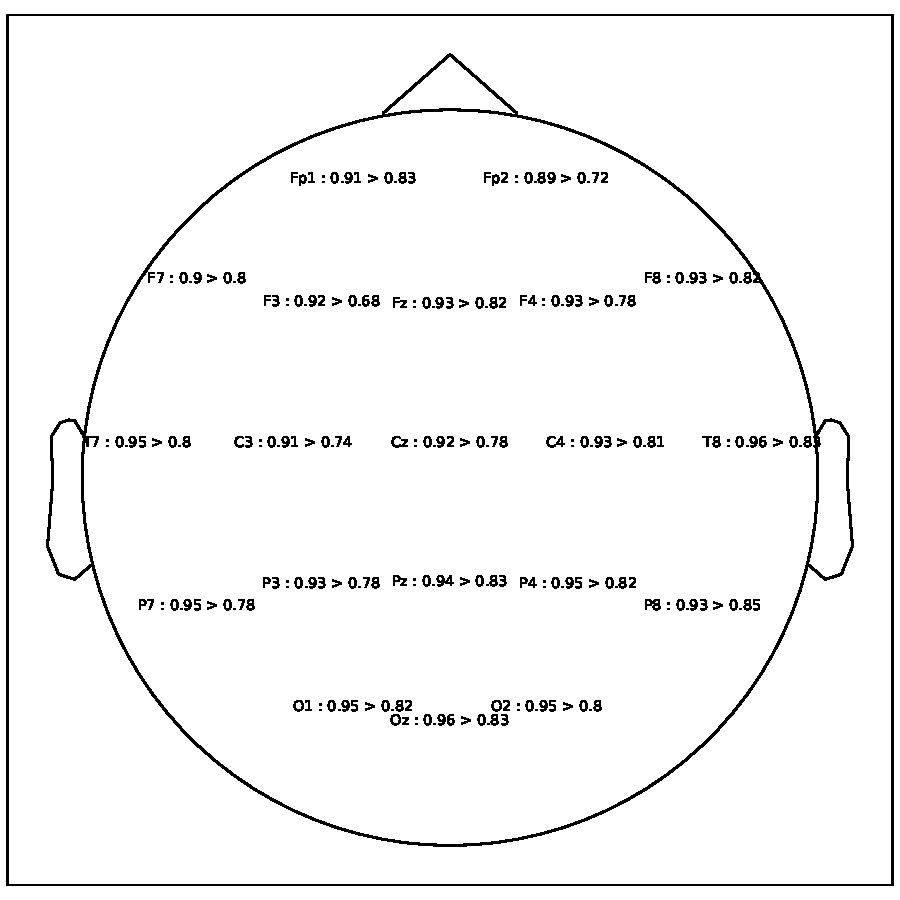
\includegraphics[width=.95\textwidth,trim={0cm 0cm 0cm 0cm},clip]{../SearchResults_1Ch/SearchSpaceResult_1Ch_20190926_S30.pdf}};
	  \begin{scope}[scale=1]
	      \draw[line width=2pt,blue] (-7.85,-7.85) node[anchor=west,right=.15cm] {\small{Best Channels according to the train accuracy}} circle (.2);
	      \draw[line width=2pt,red]  (7.85,-7.85)  node[anchor=east,left=.15cm] {\small{Best Channels according to the test accuracy}}  circle (.2);
	      %
	      \draw[line width=2pt,blue] (-.2,-5.15) node[] (OzTr) {} circle (.4);
	      \draw[line width=2pt,blue] (-2.05,-4.85) node[] (O1Tr) {} circle (.4);
	      \draw[line width=2pt,blue] (5.75, .15) node[] (T8Tr) {} circle (.4);
	      %
	      \draw[line width=2pt,red] (5.65,-2.95) node[] (P8Te) {} circle (.4);
	      \draw[line width=2pt,red] (6.7, .15) node[] (T8Te) {} circle (.4);
	      \draw[line width=2pt,red] (.8, -5.15) node[] (OzTe) {} circle (.4);
	\end{scope}
  \end{tikzpicture}
  \caption{Search for the first best channel with $30$ subjects.}
  \label{fg:1Ch_S30_B0}
\end{figure}

%%%%%%%%%%%%%%%%%%%%%%%%%%%%%%%%%%%%%%%%%%%%%%%%%%%%%%%%%%%%%%%%%%%%%%%%%%%%%%%%%%%%%%%%%%%%%%%%%%%%%%%%%%%
% SearchSpaceResult_1Ch_20190927_S30_BaselineRemovedT10
\newpage

\hspace*{12cm}\hyperlink{tab:TestResults}{(BACK TO RESULT TABLE)}

\bigskip
\bigskip

\begin{tabular}{ll}
  No. of Channels: & 1\\
  Previous Selected Channels: & --\\
  No. of Subjects: & 30\\
  Baseline Channel: & T10\\
  Task:	& REO 
\end{tabular}

\bigskip

\begin{figure}[H]
  \tikzexternaldisable
  \centering
  \begin{tikzpicture}
	  \node[inner sep=0pt] (russell) at (0,0)
	      {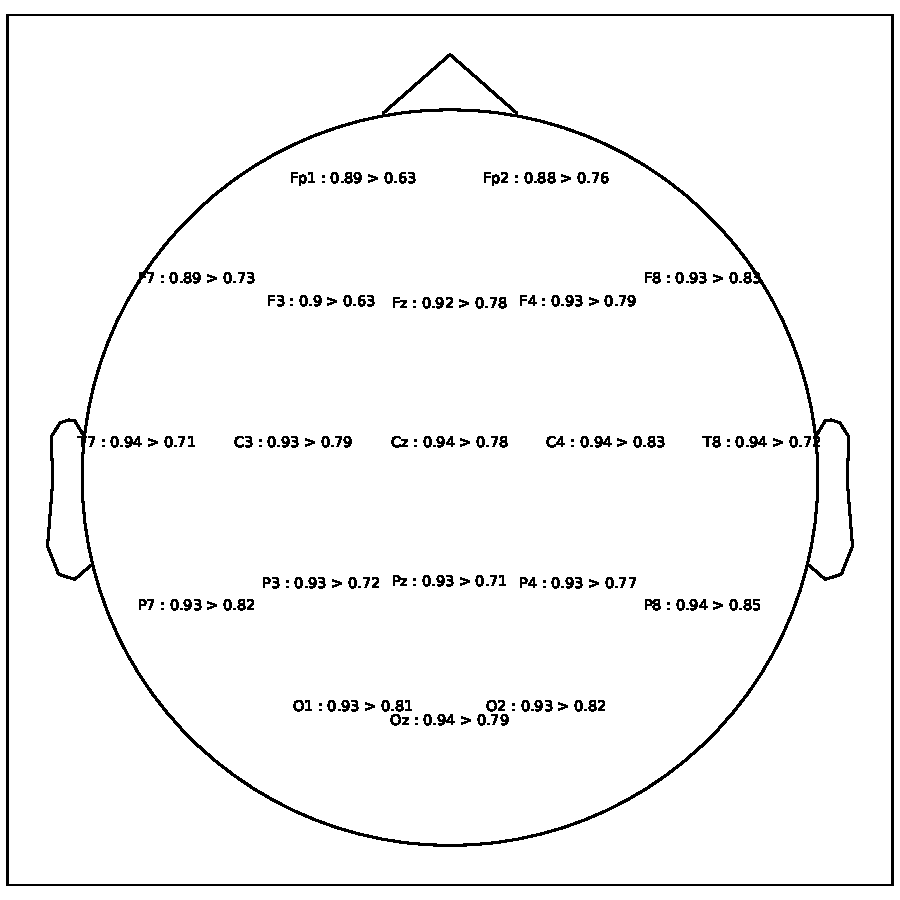
\includegraphics[width=.95\textwidth,trim={0cm 0cm 0cm 0cm},clip]{../SearchResults_1Ch/SearchSpaceResult_1Ch_20190927_S30_BaselineRemovedT10}};
	  \begin{scope}[scale=1]
	      \draw[line width=2pt,blue] (-7.85,-7.85) node[anchor=west,right=.15cm] {\small{Best Channels according to the train accuracy}} circle (.2);
	      \draw[line width=2pt,red]  (7.85,-7.85)  node[anchor=east,left=.15cm] {\small{Best Channels according to the test accuracy}}  circle (.2);
	      %
	      \draw[line width=2pt,blue] (-.2,.15) node[] (CzTr) {} circle (.4);
	      \draw[line width=2pt,blue] (2.8,.15) node[] (C4Tr) {} circle (.4);
	      \draw[line width=2pt,blue] (-.2,-5.15) node[] (OzTr) {} circle (.4);
 	      %\draw[line width=2pt,blue] (-2.05,-4.85) node[] (O1Tr) {} circle (.4);
 	      %\draw[line width=2pt,blue] (5.75, .15) node[] (T8Tr) {} circle (.4);
	      %
	      \draw[line width=2pt,red] (5.65,-2.95) node[] (P8Te) {} circle (.4);
	      \draw[line width=2pt,red] (5.6, 3.3) node[] (F8Te) {} circle (.4);
	      \draw[line width=2pt,red] (2.8+1, .15) node[] (C4Te) {} circle (.4);
 	      %\draw[line width=2pt,red] (6.7, .15) node[] (T8Te) {} circle (.4);
 	      %\draw[line width=2pt,red] (.8, -5.15) node[] (OzTe) {} circle (.4);
	\end{scope}
  \end{tikzpicture}
  \caption{Search for the first best channel with $30$ subjects, T10 is removed as baseline.}
  \label{fg:1Ch_S30_B1}
\end{figure}


%%%%%%%%%%%%%%%%%%%%%%%%%%%%%%%%%%%%%%%%%%%%%%%%%%%%%%%%%%%%%%%%%%%%%%%%%%%%%%%%%%%%%%%%%%%%%%%%%%%%%%%%%%%
% SearchSpaceResult_1Ch_S40_RemoveBaseLineOff_20191008
\newpage

\hspace*{12cm}\hyperlink{tab:TestResults}{(BACK TO RESULT TABLE)}

\bigskip
\bigskip

\begin{tabular}{ll}
  No. of Channels: & 1\\
  Previous Selected Channels: & --\\
  No. of Subjects: & 40\\
  Baseline Channel: & --\\
  Task:	& REO 
\end{tabular}

\bigskip

\begin{figure}[H]
  \tikzexternaldisable
  \centering
  \begin{tikzpicture}
	  \node[inner sep=0pt] (russell) at (0,0)
	      {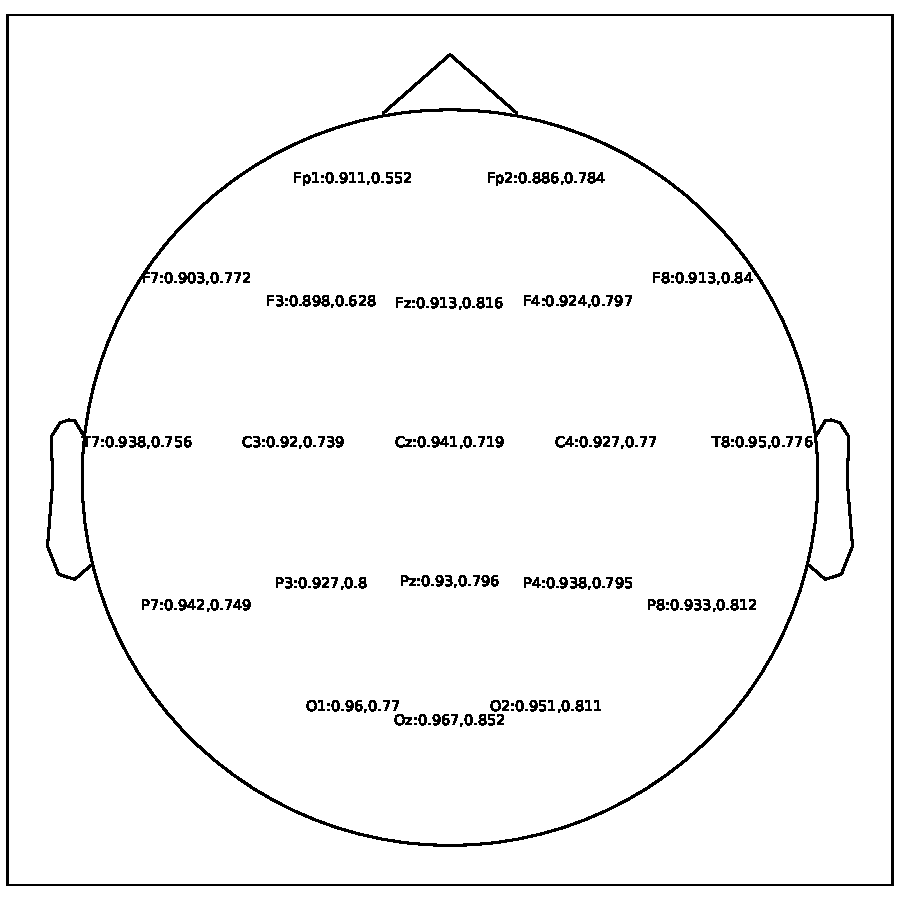
\includegraphics[width=.95\textwidth,trim={0cm 0cm 0cm 0cm},clip]{../SearchResults_1Ch/SearchSpaceResult_1Ch_S40_RemoveBaseLineOff_20191008}};
	  \begin{scope}[scale=1]
	      \draw[line width=2pt,blue] (-7.85,-7.85) node[anchor=west,right=.15cm] {\small{Best Channels according to the train accuracy}} circle (.2);
	      \draw[line width=2pt,red]  (7.85,-7.85)  node[anchor=east,left=.15cm] {\small{Best Channels according to the test accuracy}}  circle (.2);
	      %
	      \draw[line width=2pt,blue] (-.2,-5.1) node[] (OzTr) {} circle (.45);
 	      \draw[line width=2pt,blue] (1.65,-4.9) node[] (O2Tr) {} circle (.45);
 	      %\draw[line width=2pt,blue] (-6.1,.15) node[] (T7Tr) {} circle (.45);
 	      %\draw[line width=2pt,blue] (-.2,.15) node[] (CzTr) {} circle (.4);
	      %\draw[line width=2pt,blue] (2.8,.15) node[] (C4Tr) {} circle (.4);
	      \draw[line width=2pt,blue] (-1.9,-4.9) node[] (O1Tr) {} circle (.4);
 	      %\draw[line width=2pt,blue] (-2.05,-4.85) node[] (O1Tr) {} circle (.4);
 	      %\draw[line width=2pt,blue] (5.75, .15) node[] (T8Tr) {} circle (.45);
	      %\draw[line width=2pt,blue] (4.6, 3.25) node[] (F8Tr) {} circle (.45);
	      %\draw[line width=2pt,blue] (2.2, 2.85) node[] (F4Tr) {} circle (.45);
	      %\draw[line width=2pt,blue] (-.25, 2.8) node[] (FzTr) {} circle (.45);
	      %\draw[line width=2pt,blue] (-5., -2.95) node[] (P7Tr) {} circle (.45);
	      %\draw[line width=2pt,blue] (4.6, -2.95) node[] (P8Tr) {} circle (.45);
	      %\draw[line width=2pt,blue] (-.25, -2.5) node[] (PzTr) {} circle (.45);
	      %
	      \draw[line width=2pt,red] (.6,2.8) node[] (FzTe) {} circle (.45);
	      %\draw[line width=2pt,red] (3.1, 2.85) node[] (F4Te) {} circle (.45);
	      %\draw[line width=2pt,red] (3.1,-2.5) node[] (P4Te) {} circle (.45);
	      %\draw[line width=2pt,red] (.6,-2.5) node[] (PzTe) {} circle (.45);
	      %\draw[line width=2pt,red] (5.4,-2.95) node[] (P8Te) {} circle (.45);
	      \draw[line width=2pt,red] (5.45, 3.25) node[] (F8Te) {} circle (.45);
	      %\draw[line width=2pt,red] (-1.25, -4.85) node[] (O1Te) {} circle (.45);
	      %\draw[line width=2pt,red] (-2.3, .15) node[] (C3Te) {} circle (.45);
	      %\draw[line width=2pt,red] (.65, .15) node[] (CzTe) {} circle (.45);
 	      %\draw[line width=2pt,red] (2.8+1, .15) node[] (C4Te) {} circle (.4);
 	      %\draw[line width=2pt,red] (6.65, .15) node[] (T8Te) {} circle (.4);
 	      \draw[line width=2pt,red] (.7, -5.1) node[] (OzTe) {} circle (.45);
	\end{scope}
  \end{tikzpicture}
  \caption{Search for the first best channel with $40$ subjects, no baseline is removed.}
  \label{fg:1Ch_S40_B0}
\end{figure}


%%%%%%%%%%%%%%%%%%%%%%%%%%%%%%%%%%%%%%%%%%%%%%%%%%%%%%%%%%%%%%%%%%%%%%%%%%%%%%%%%%%%%%%%%%%%%%%%%%%%%%%%%%%
% SearchSpaceResult_1Ch_S40_RemoveBaseLineOn_20191011
\newpage

\hspace*{12cm}\hyperlink{tab:TestResults}{(BACK TO RESULT TABLE)}

\bigskip
\bigskip

\begin{tabular}{ll}
  No. of Channels: & 1\\
  Previous Selected Channels: & --\\
  No. of Subjects: & 40\\
  Baseline Channel: & T10\\
  Task:	& REO 
\end{tabular}

\bigskip

\begin{figure}[H]
  \tikzexternaldisable
  \centering
  \begin{tikzpicture}
	  \node[inner sep=0pt] (russell) at (0,0)
	      {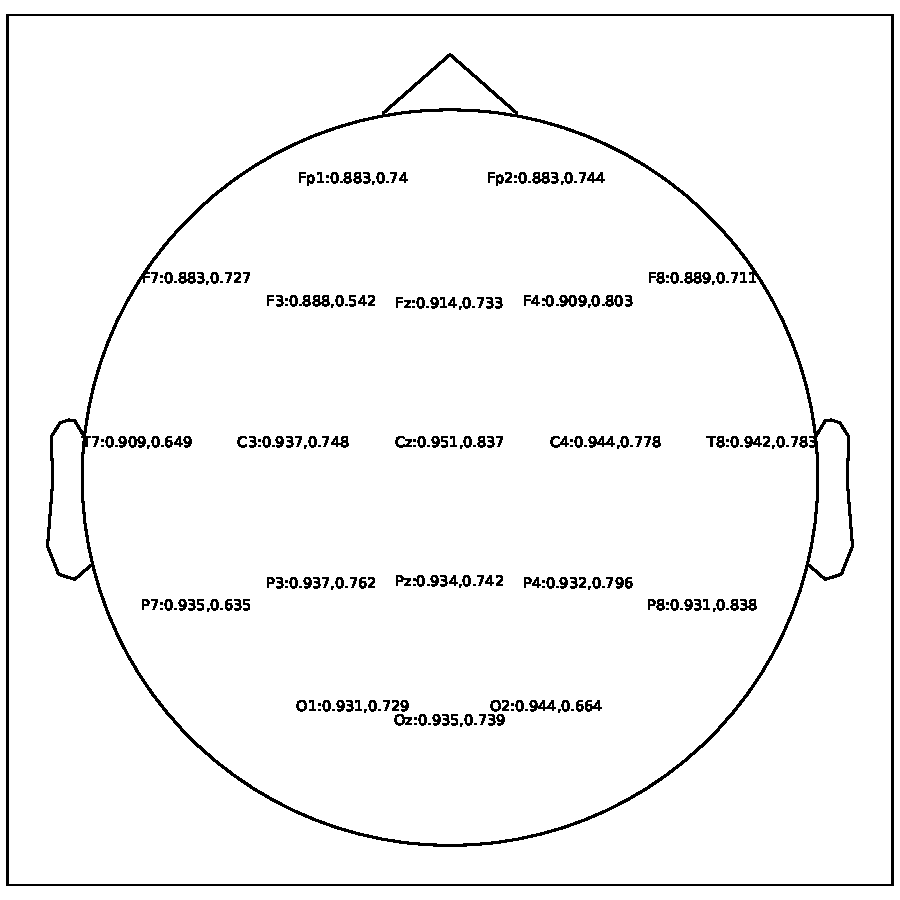
\includegraphics[width=.95\textwidth,trim={0cm 0cm 0cm 0cm},clip]{../SearchResults_1Ch/SearchSpaceResult_1Ch_S40_RemoveBaseLineOn_20191011}};
	  \begin{scope}[scale=1]
	      \draw[line width=2pt,blue] (-7.85,-7.85) node[anchor=west,right=.15cm] {\small{Best Channels according to the train accuracy}} circle (.2);
	      \draw[line width=2pt,red]  (7.85,-7.85)  node[anchor=east,left=.15cm] {\small{Best Channels according to the test accuracy}}  circle (.2);
	      %
	      %\draw[line width=2pt,blue] (-.2,-5.1) node[] (OzTr) {} circle (.45);
 	      \draw[line width=2pt,blue] (1.65,-4.9) node[] (O2Tr) {} circle (.45);
 	      %\draw[line width=2pt,blue] (-6.1,.15) node[] (T7Tr) {} circle (.45);
	      \draw[line width=2pt,blue] (-.25,.15) node[] (CzTr) {} circle (.45);
	      \draw[line width=2pt,blue] (2.75,.15) node[] (C4Tr) {} circle (.45);
	      %\draw[line width=2pt,blue] (-3.2,.15) node[] (C3Tr) {} circle (.45);
	      %\draw[line width=2pt,blue] (-2.05,-4.9) node[] (O1Tr) {} circle (.45);
 	      %\draw[line width=2pt,blue] (-2.05,-4.85) node[] (O1Tr) {} circle (.4);
 	      %\draw[line width=2pt,blue] (5.75, .15) node[] (T8Tr) {} circle (.45);
	      %\draw[line width=2pt,blue] (4.6, 3.25) node[] (F8Tr) {} circle (.45);
	      %\draw[line width=2pt,blue] (2.2, 2.85) node[] (F4Tr) {} circle (.45);
	      %\draw[line width=2pt,blue] (-.25, 2.8) node[] (FzTr) {} circle (.45);
	      %\draw[line width=2pt,blue] (-5., -2.95) node[] (P7Tr) {} circle (.45);
	      %\draw[line width=2pt,blue] (-2., 5.2) node[] (PF1Tr) {} circle (.45);
	      %\draw[line width=2pt,blue] (1.7, 5.2) node[] (PF2Tr) {} circle (.45);
	      %\draw[line width=2pt,blue] (4.6, -2.95) node[] (P8Tr) {} circle (.45);
	      %\draw[line width=2pt,blue] (-.25, -2.5) node[] (PzTr) {} circle (.45);
	      %
	      %\draw[line width=2pt,red] (.6,2.8) node[] (FzTe) {} circle (.45);
	      %\draw[line width=2pt,red] (3.1, 2.85) node[] (F4Te) {} circle (.45);
	      \draw[line width=2pt,red] (3.1,-2.5) node[] (P4Te) {} circle (.45);
	      %\draw[line width=2pt,red] (.6,-2.5) node[] (PzTe) {} circle (.45);
	      \draw[line width=2pt,red] (5.45,-2.95) node[] (P8Te) {} circle (.45);
	      %\draw[line width=2pt,red] (2.55,5.2) node[] (FP2Te) {} circle (.45);
	      %\draw[line width=2pt,red] (5.45, 3.25) node[] (F8Te) {} circle (.45);
	      %\draw[line width=2pt,red] (-4.15, 3.25) node[] (F7Te) {} circle (.45);
	      %\draw[line width=2pt,red] (-1.25, -4.85) node[] (O1Te) {} circle (.45);
	      %\draw[line width=2pt,red] (-2.3, .15) node[] (C3Te) {} circle (.45);
	      \draw[line width=2pt,red] (.65, .15) node[] (CzTe) {} circle (.45);
 	      %\draw[line width=2pt,red] (2.8+1, .15) node[] (C4Te) {} circle (.4);
	      %\draw[line width=2pt,red] (6.6, .15) node[] (T8Te) {} circle (.45);
 	      %\draw[line width=2pt,red] (.7, -5.1) node[] (OzTe) {} circle (.45);
	\end{scope}
  \end{tikzpicture}
  \caption{Search for the first best channel with $40$ subjects, T10 is removed as baseline.}
  \label{fg:1Ch_S40_B1}
\end{figure}



%%%%%%%%%%%%%%%%%%%%%%%%%%%%%%%%%%%%%%%%%%%%%%%%%%%%%%%%%%%%%%%%%%%%%%%%%%%%%%%%%%%%%%%%%%%%%%%%%%%%%%%%%%%
% SearchSpaceResult_1Ch_20191003_S50
\newpage

\hspace*{12cm}\hyperlink{tab:TestResults}{(BACK TO RESULT TABLE)}

\bigskip
\bigskip

\begin{tabular}{ll}
  No. of Channels: & 1\\
  Previous Selected Channels: & --\\
  No. of Subjects: & 50\\
  Baseline Channel: & --\\
  Task:	& REO 
\end{tabular}

\bigskip

\begin{figure}[H]
  \tikzexternaldisable
  \centering
  \begin{tikzpicture}
	  \node[inner sep=0pt] (russell) at (0,0)
	      {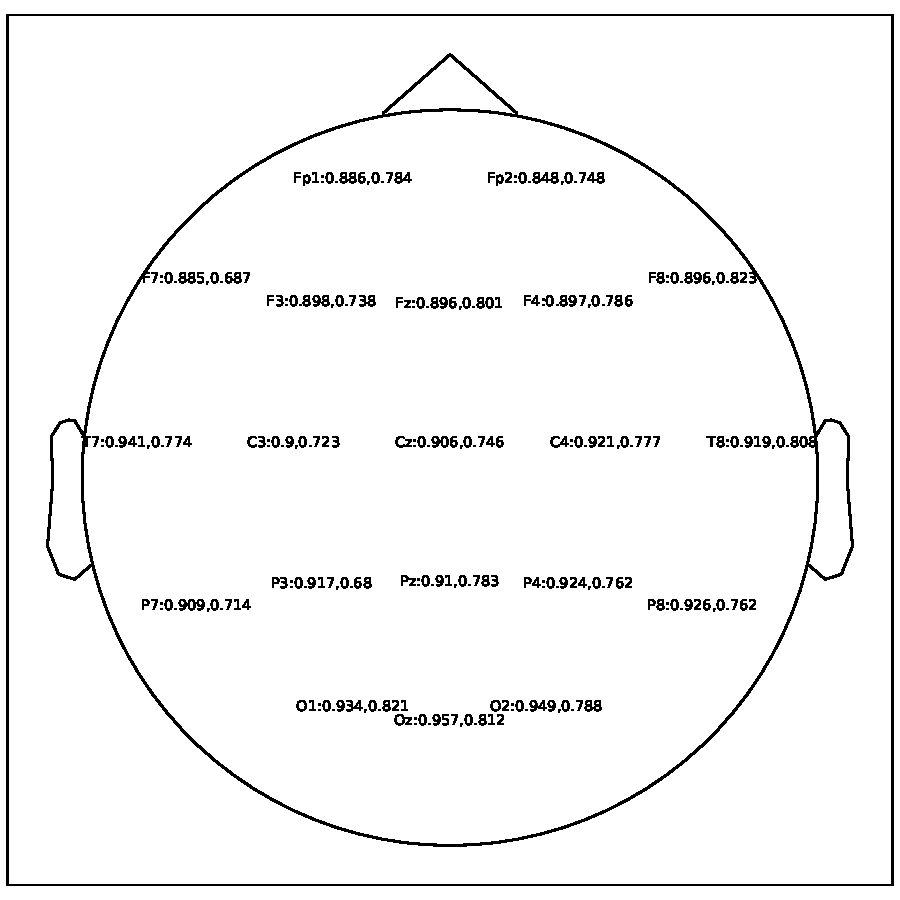
\includegraphics[width=.95\textwidth,trim={0cm 0cm 0cm 0cm},clip]{../SearchResults_1Ch/SearchSpaceResult_1Ch_20191003_S50}};
	  \begin{scope}[scale=1]
	      \draw[line width=2pt,blue] (-7.85,-7.85) node[anchor=west,right=.15cm] {\small{Best Channels according to the train accuracy}} circle (.2);
	      \draw[line width=2pt,red]  (7.85,-7.85)  node[anchor=east,left=.15cm] {\small{Best Channels according to the test accuracy}}  circle (.2);
	      %
	      \draw[line width=2pt,blue] (-.2,-5.15) node[] (OzTr) {} circle (.45);
 	      \draw[line width=2pt,blue] (1.65,-4.9) node[] (O2Tr) {} circle (.45);
 	      \draw[line width=2pt,blue] (-6.15,.15) node[] (T7Tr) {} circle (.45);
 	      %\draw[line width=2pt,blue] (-.2,.15) node[] (CzTr) {} circle (.4);
	      %\draw[line width=2pt,blue] (2.8,.15) node[] (C4Tr) {} circle (.4);
	      %\draw[line width=2pt,blue] (-.2,-5.15) node[] (OzTr) {} circle (.4);
 	      %\draw[line width=2pt,blue] (-2.05,-4.85) node[] (O1Tr) {} circle (.4);
 	      %\draw[line width=2pt,blue] (5.75, .15) node[] (T8Tr) {} circle (.4);
	      %
	      %\draw[line width=2pt,red] (5.65,-2.95) node[] (P8Te) {} circle (.4);
	      \draw[line width=2pt,red] (5.45, 3.25) node[] (F8Te) {} circle (.45);
	      \draw[line width=2pt,red] (-1.2, -4.9) node[] (O1Te) {} circle (.45);
	      %\draw[line width=2pt,red] (2.8+1, .15) node[] (C4Te) {} circle (.4);
 	      %\draw[line width=2pt,red] (6.7, .15) node[] (T8Te) {} circle (.4);
 	      \draw[line width=2pt,red] (.7, -5.15) node[] (OzTe) {} circle (.45);
	\end{scope}
  \end{tikzpicture}
  \caption{Search for the first best channel with $30$ subjects, no baseline removed.}
  \label{fg:1Ch_S50_B0}
\end{figure}


%%%%%%%%%%%%%%%%%%%%%%%%%%%%%%%%%%%%%%%%%%%%%%%%%%%%%%%%%%%%%%%%%%%%%%%%%%%%%%%%%%%%%%%%%%%%%%%%%%%%%%%%%%%
% SearchSpaceResult_1Ch_S50_RemoveBaseLineOn_20191011
\newpage

\hspace*{12cm}\hyperlink{tab:TestResults}{(BACK TO RESULT TABLE)}

\bigskip
\bigskip

\begin{tabular}{ll}
  No. of Channels: & 1\\
  Previous Selected Channels: & ---\\
  No. of Subjects: & 50\\
  Baseline Channel: & T10\\
  Task:	& REO 
\end{tabular}

\bigskip

\begin{figure}[H]
  \tikzexternaldisable
  \centering
  \begin{tikzpicture}
	  \node[inner sep=0pt] (russell) at (0,0)
	      {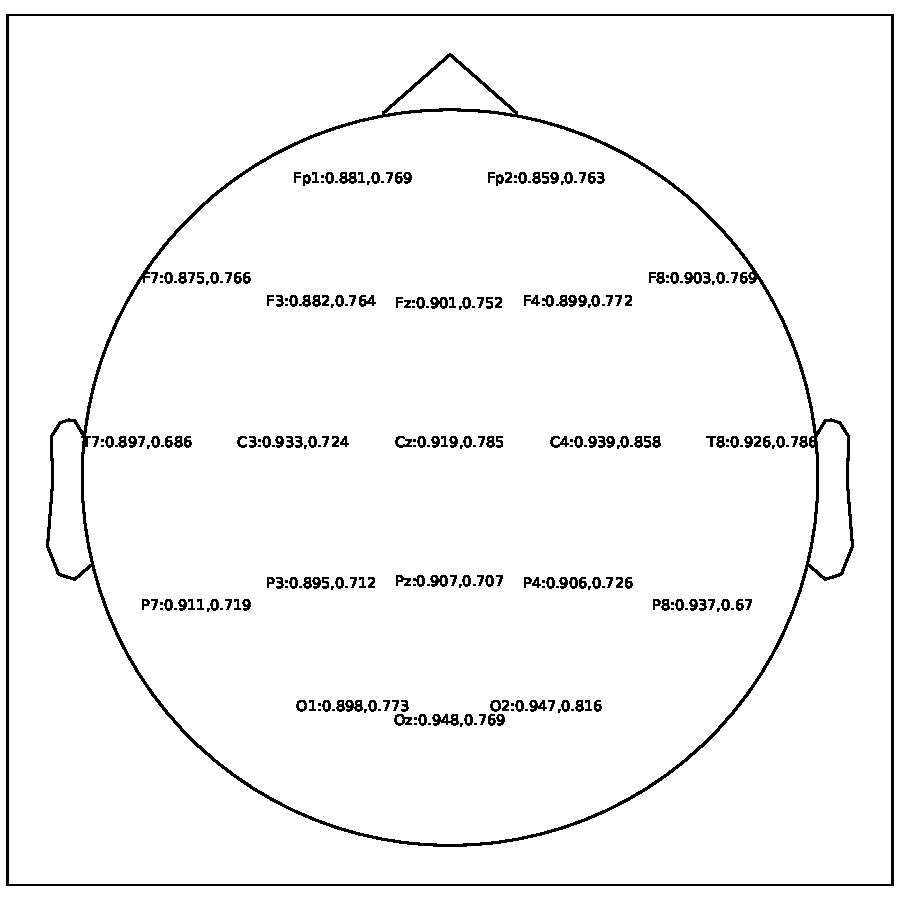
\includegraphics[width=.95\textwidth,trim={0cm 0cm 0cm 0cm},clip]{../SearchResults_1Ch/SearchSpaceResult_1Ch_S50_RemoveBaseLineOn_20191011}};
	  \begin{scope}[scale=1]
	      \draw[line width=2pt,blue] (-7.85,-7.85) node[anchor=west,right=.15cm] {\small{Best Channels according to the train accuracy}} circle (.2);
	      \draw[line width=2pt,red]  (7.85,-7.85)  node[anchor=east,left=.15cm] {\small{Best Channels according to the test accuracy}}  circle (.2);
	      %
	      \draw[line width=2pt,blue] (-.2,-5.1) node[] (OzTr) {} circle (.45);
 	      \draw[line width=2pt,blue] (1.65,-4.85) node[] (O2Tr) {} circle (.45);
 	      %\draw[line width=2pt,blue] (-6.1,.15) node[] (T7Tr) {} circle (.45);
	      %\draw[line width=2pt,blue] (-.25,.15) node[] (CzTr) {} circle (.45);
	      \draw[line width=2pt,blue] (2.75,.15) node[] (C4Tr) {} circle (.45);
	      %\draw[line width=2pt,blue] (-3.2,.15) node[] (C3Tr) {} circle (.45);
	      %\draw[line width=2pt,blue] (-2.05,-4.9) node[] (O1Tr) {} circle (.45);
 	      %\draw[line width=2pt,blue] (5.75, .15) node[] (T8Tr) {} circle (.45);
	      %\draw[line width=2pt,blue] (4.6, 3.25) node[] (F8Tr) {} circle (.45);
	      %\draw[line width=2pt,blue] (2.2, 2.85) node[] (F4Tr) {} circle (.45);
	      %\draw[line width=2pt,blue] (-.25, 2.8) node[] (FzTr) {} circle (.45);
	      %\draw[line width=2pt,blue] (-5., -2.95) node[] (P7Tr) {} circle (.45);
	      %\draw[line width=2pt,blue] (-2., 5.2) node[] (PF1Tr) {} circle (.45);
	      %\draw[line width=2pt,blue] (1.7, 5.2) node[] (PF2Tr) {} circle (.45);
	      %\draw[line width=2pt,blue] (4.6, -2.95) node[] (P8Tr) {} circle (.45);
	      %\draw[line width=2pt,blue] (-2.7, -2.5) node[] (P3Tr) {} circle (.45);
	      %\draw[line width=2pt,blue] (-.25, -2.5) node[] (PzTr) {} circle (.45);
	      %
	      %\draw[line width=2pt,red] (.6,2.8) node[] (FzTe) {} circle (.45);
	      %\draw[line width=2pt,red] (3.1, 2.85) node[] (F4Te) {} circle (.45);
	      %\draw[line width=2pt,red] (3.1,-2.5) node[] (P4Te) {} circle (.45);
	      %\draw[line width=2pt,red] (.6,-2.5) node[] (PzTe) {} circle (.45);
	      %\draw[line width=2pt,red] (5.45,-2.95) node[] (P8Te) {} circle (.45);
	      %\draw[line width=2pt,red] (2.55,5.2) node[] (FP2Te) {} circle (.45);
	      %\draw[line width=2pt,red] (5.45, 3.25) node[] (F8Te) {} circle (.45);
	      %\draw[line width=2pt,red] (-4.15, 3.25) node[] (F7Te) {} circle (.45);
	      %\draw[line width=2pt,red] (-1.25, -4.85) node[] (O1Te) {} circle (.45);
	      \draw[line width=2pt,red] (2.65, -4.85) node[] (O2Te) {} circle (.45);
	      %\draw[line width=2pt,red] (-2.3, .15) node[] (C3Te) {} circle (.45);
	      %\draw[line width=2pt,red] (.65, .15) node[] (CzTe) {} circle (.45);
 	      \draw[line width=2pt,red] (2.8+1, .15) node[] (C4Te) {} circle (.45);
	      \draw[line width=2pt,red] (6.6, .15) node[] (T8Te) {} circle (.45);
 	      %\draw[line width=2pt,red] (.7, -5.1) node[] (OzTe) {} circle (.45);
	\end{scope}
  \end{tikzpicture}
  \caption{Search for the first best channel with $50$ subjects, T10 is removed as baseline.}
  \label{fg:1Ch_S50_B1}
\end{figure}


%%%%%%%%%%%%%%%%%%%%%%%%%%%%%%%%%%%%%%%%%%%%%%%%%%%%%%%%%%%%%%%%%%%%%%%%%%%%%%%%%%%%%%%%%%%%%%%%%%%%%%%%%%%
% SearchSpaceResult_2Ch_(61)_S30_RemoveBaseLineOff_20190927_Try1
\newpage

\hspace*{12cm}\hyperlink{tab:TestResults}{(BACK TO RESULT TABLE)}

\bigskip
\bigskip

\begin{tabular}{ll}
  No. of Channels: & 2\\
  Previous Selected Channels: & Oz\\
  No. of Subjects: & 30\\
  Baseline Channel: & --\\
  Task:	& REO 
\end{tabular}

\bigskip

\begin{figure}[H]
  \tikzexternaldisable
  \centering
  \begin{tikzpicture}
	  \node[inner sep=0pt] (russell) at (0,0)
	      {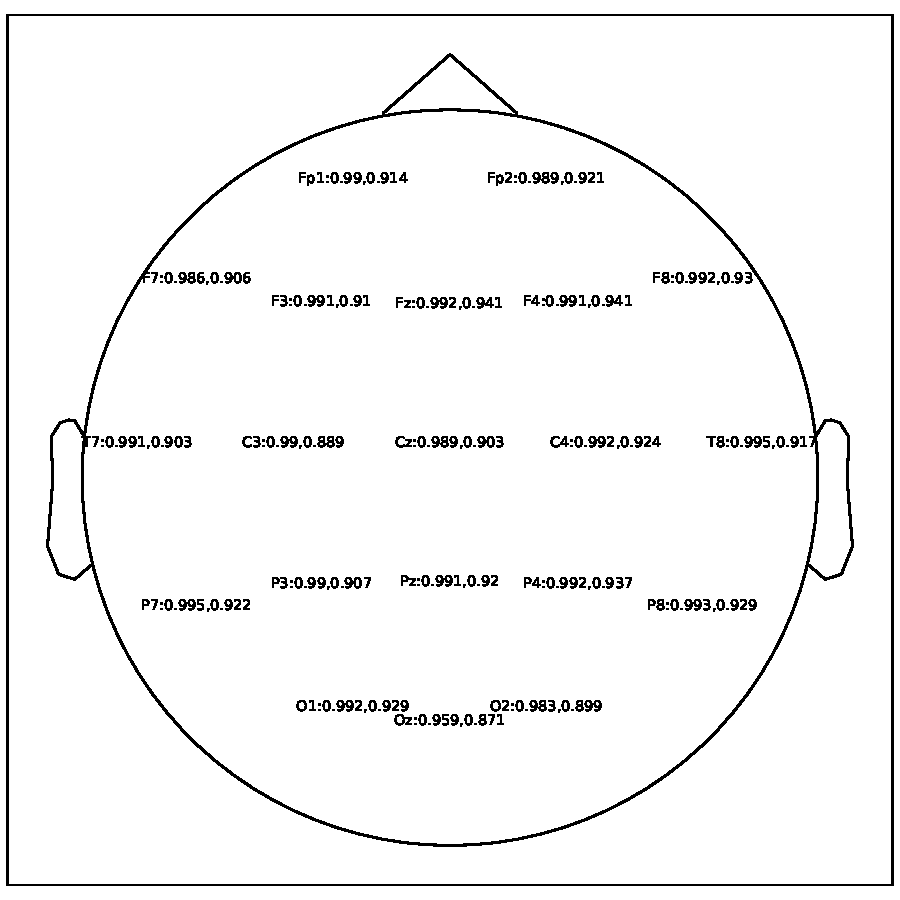
\includegraphics[width=.95\textwidth,trim={0cm 0cm 0cm 0cm},clip]{../SearchResults_2Ch/SearchSpaceResult_2Ch_(61)_S30_RemoveBaseLineOff_20190927_Try1}};
	  \begin{scope}[scale=1]
	      \draw[line width=2pt,blue] (-7.85,-7.85) node[anchor=west,right=.15cm] {\small{Best Channels according to the train accuracy}} circle (.2);
	      \draw[line width=2pt,red]  (7.85,-7.85)  node[anchor=east,left=.15cm] {\small{Best Channels according to the test accuracy}}  circle (.2);
	      %
	      %\draw[line width=2pt,blue] (-.2,-5.15) node[] (OzTr) {} circle (.45);
 	      %\draw[line width=2pt,blue] (1.65,-4.9) node[] (O2Tr) {} circle (.45);
 	      %\draw[line width=2pt,blue] (-6.15,.15) node[] (T7Tr) {} circle (.45);
 	      %\draw[line width=2pt,blue] (-.2,.15) node[] (CzTr) {} circle (.4);
	      %\draw[line width=2pt,blue] (2.8,.15) node[] (C4Tr) {} circle (.4);
	      %\draw[line width=2pt,blue] (-.2,-5.15) node[] (OzTr) {} circle (.4);
 	      %\draw[line width=2pt,blue] (-2.05,-4.85) node[] (O1Tr) {} circle (.4);
 	      \draw[line width=2pt,blue] (5.75, .15) node[] (T8Tr) {} circle (.45);
	      \draw[line width=2pt,blue] (-5., -2.95) node[] (P7Tr) {} circle (.45);
	      \draw[line width=2pt,blue] (4.6, -2.95) node[] (P8Tr) {} circle (.45);
	      %
	      \draw[line width=2pt,red] (.6,2.8) node[] (FzTe) {} circle (.45);
	      \draw[line width=2pt,red] (3.1, 2.8) node[] (F4Te) {} circle (.45);
	      \draw[line width=2pt,red] (3.1,-2.5) node[] (P4Te) {} circle (.45);
	      %\draw[line width=2pt,red] (5.65,-2.95) node[] (P8Te) {} circle (.4);
	      %\draw[line width=2pt,red] (5.45, 3.25) node[] (F8Te) {} circle (.45);
	      %\draw[line width=2pt,red] (-1.2, -4.9) node[] (O1Te) {} circle (.45);
	      %\draw[line width=2pt,red] (2.8+1, .15) node[] (C4Te) {} circle (.4);
 	      %\draw[line width=2pt,red] (6.7, .15) node[] (T8Te) {} circle (.4);
 	      %\draw[line width=2pt,red] (.7, -5.15) node[] (OzTe) {} circle (.45);
	\end{scope}
  \end{tikzpicture}
  \caption{Search for the second best channel with $30$ subjects, no baseline removed.}
  \label{fg:2Ch_S30_B0}
\end{figure}

%%%%%%%%%%%%%%%%%%%%%%%%%%%%%%%%%%%%%%%%%%%%%%%%%%%%%%%%%%%%%%%%%%%%%%%%%%%%%%%%%%%%%%%%%%%%%%%%%%%%%%%%%%%
% SearchSpaceResult_2Ch_(61)_S30_RemoveBaseLineOn_T10_20190929
\newpage

\hspace*{12cm}\hyperlink{tab:TestResults}{(BACK TO RESULT TABLE)}

\bigskip
\bigskip

\begin{tabular}{ll}
  No. of Channels: & 2\\
  Previous Selected Channels: & Oz\\
  No. of Subjects: & 30\\
  Baseline Channel: & T10\\
  Task:	& REO 
\end{tabular}

\bigskip

\begin{figure}[H]
  \tikzexternaldisable
  \centering
  \begin{tikzpicture}
	  \node[inner sep=0pt] (russell) at (0,0)
	      {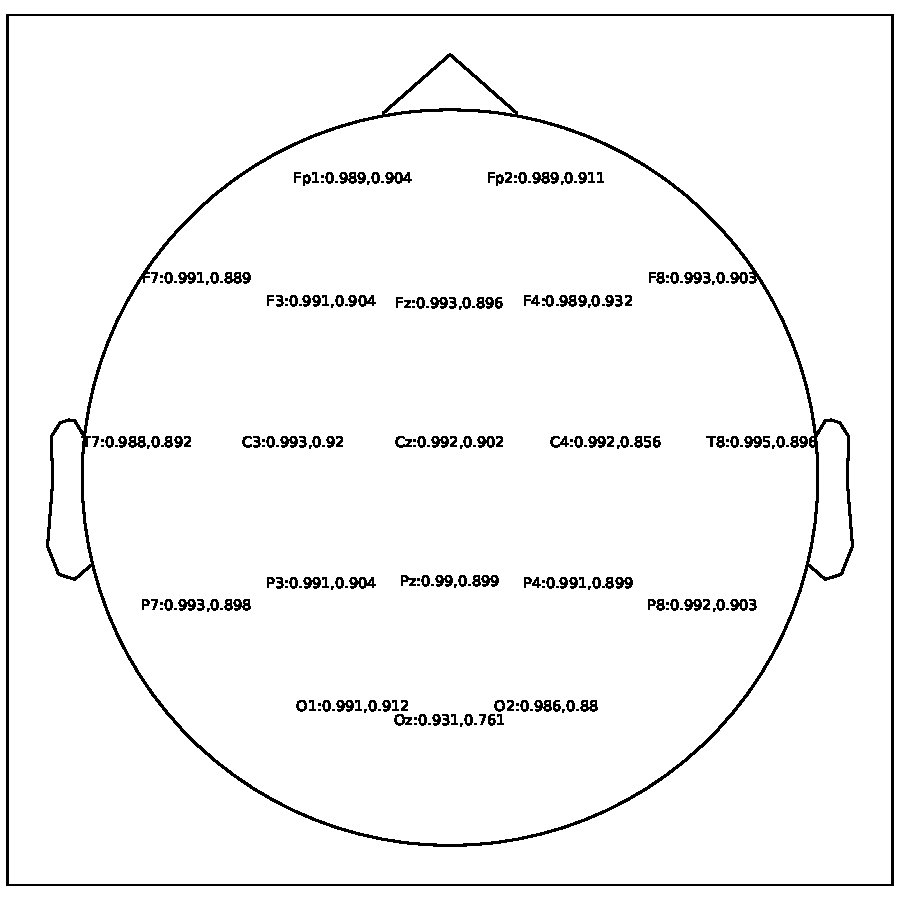
\includegraphics[width=.95\textwidth,trim={0cm 0cm 0cm 0cm},clip]{../SearchResults_2Ch/SearchSpaceResult_2Ch_(61)_S30_RemoveBaseLineOn_T10_20190929}};
	  \begin{scope}[scale=1]
	      \draw[line width=2pt,blue] (-7.85,-7.85) node[anchor=west,right=.15cm] {\small{Best Channels according to the train accuracy}} circle (.2);
	      \draw[line width=2pt,red]  (7.85,-7.85)  node[anchor=east,left=.15cm] {\small{Best Channels according to the test accuracy}}  circle (.2);
	      %
	      %\draw[line width=2pt,blue] (-.2,-5.15) node[] (OzTr) {} circle (.45);
 	      %\draw[line width=2pt,blue] (1.65,-4.9) node[] (O2Tr) {} circle (.45);
 	      %\draw[line width=2pt,blue] (-6.15,.15) node[] (T7Tr) {} circle (.45);
 	      %\draw[line width=2pt,blue] (-.2,.15) node[] (CzTr) {} circle (.4);
	      %\draw[line width=2pt,blue] (2.8,.15) node[] (C4Tr) {} circle (.4);
	      %\draw[line width=2pt,blue] (-.2,-5.15) node[] (OzTr) {} circle (.4);
 	      %\draw[line width=2pt,blue] (-2.05,-4.85) node[] (O1Tr) {} circle (.4);
 	      \draw[line width=2pt,blue] (5.75, .15) node[] (T8Tr) {} circle (.45);
		\draw[line width=2pt,blue] (4.6, 3.25) node[] (F8Tr) {} circle (.45);
	      \draw[line width=2pt,blue] (-5., -2.95) node[] (P7Tr) {} circle (.45);
	      %\draw[line width=2pt,blue] (4.6, -2.95) node[] (P8Tr) {} circle (.45);
	      %
	      %\draw[line width=2pt,red] (.6,2.8) node[] (FzTe) {} circle (.45);
	      \draw[line width=2pt,red] (3.1, 2.85) node[] (F4Te) {} circle (.45);
	      %\draw[line width=2pt,red] (3.1,-2.5) node[] (P4Te) {} circle (.45);
	      %\draw[line width=2pt,red] (5.65,-2.95) node[] (P8Te) {} circle (.4);
	      %\draw[line width=2pt,red] (5.45, 3.25) node[] (F8Te) {} circle (.45);
	      \draw[line width=2pt,red] (-1.2, -4.85) node[] (O1Te) {} circle (.45);
		\draw[line width=2pt,red] (-2.3, .15) node[] (C3Te) {} circle (.45);
 	      %\draw[line width=2pt,red] (2.8+1, .15) node[] (C4Te) {} circle (.4);
 	      %\draw[line width=2pt,red] (6.7, .15) node[] (T8Te) {} circle (.4);
 	      %\draw[line width=2pt,red] (.7, -5.15) node[] (OzTe) {} circle (.45);
	\end{scope}
  \end{tikzpicture}
  \caption{Search for the second best channel with $30$ subjects, T10 is removed as baseline.}
  \label{fg:2Ch_S30_B1}
\end{figure}

%%%%%%%%%%%%%%%%%%%%%%%%%%%%%%%%%%%%%%%%%%%%%%%%%%%%%%%%%%%%%%%%%%%%%%%%%%%%%%%%%%%%%%%%%%%%%%%%%%%%%%%%%%%
% SearchSpaceResult_2Ch_(61)_S40_RemoveBaseLineOff_20191004
\newpage

\hspace*{12cm}\hyperlink{tab:TestResults}{(BACK TO RESULT TABLE)}

\bigskip
\bigskip

\begin{tabular}{ll}
  No. of Channels: & 2\\
  Previous Selected Channels: & Oz\\
  No. of Subjects: & 40\\
  Baseline Channel: & --\\
  Task:	& REO 
\end{tabular}

\bigskip

\begin{figure}[H]
  \tikzexternaldisable
  \centering
  \begin{tikzpicture}
	  \node[inner sep=0pt] (russell) at (0,0)
	      {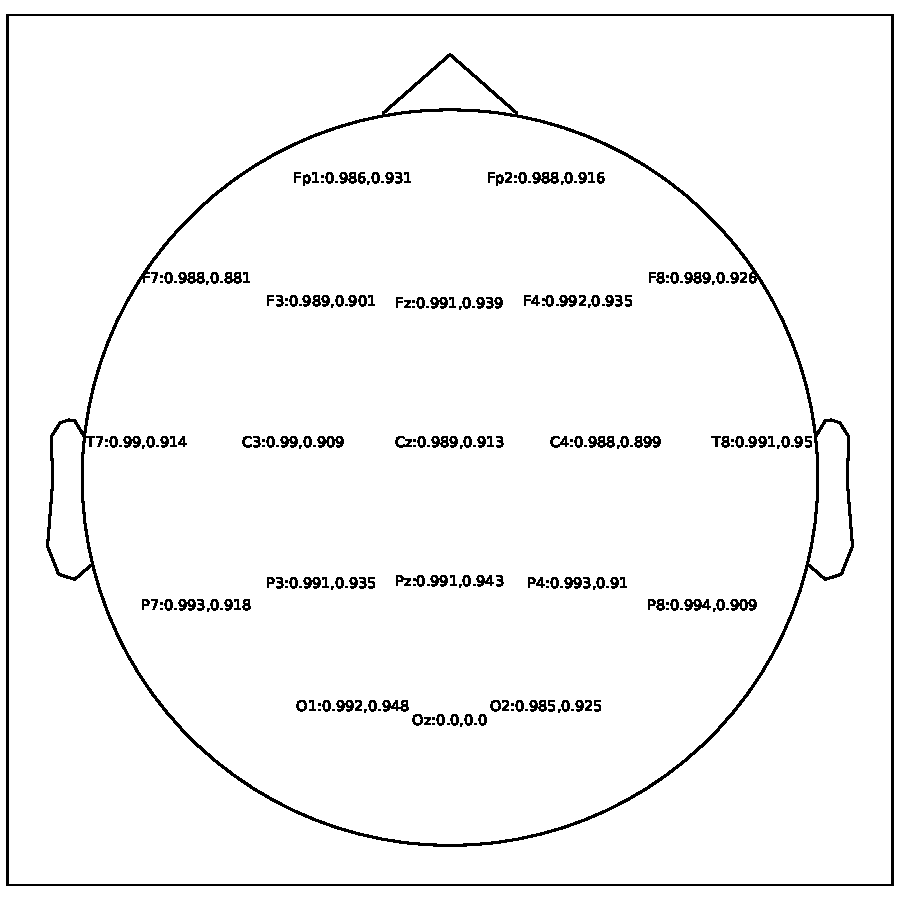
\includegraphics[width=.95\textwidth,trim={0cm 0cm 0cm 0cm},clip]{../SearchResults_2Ch/SearchSpaceResult_2Ch_(61)_S40_RemoveBaseLineOff_20191004}};
	  \begin{scope}[scale=1]
	      \draw[line width=2pt,blue] (-7.85,-7.85) node[anchor=west,right=.15cm] {\small{Best Channels according to the train accuracy}} circle (.2);
	      \draw[line width=2pt,red]  (7.85,-7.85)  node[anchor=east,left=.15cm] {\small{Best Channels according to the test accuracy}}  circle (.2);
	      %
	      %\draw[line width=2pt,blue] (-.2,-5.15) node[] (OzTr) {} circle (.45);
 	      %\draw[line width=2pt,blue] (1.65,-4.9) node[] (O2Tr) {} circle (.45);
 	      %\draw[line width=2pt,blue] (-6.15,.15) node[] (T7Tr) {} circle (.45);
 	      %\draw[line width=2pt,blue] (-.2,.15) node[] (CzTr) {} circle (.4);
	      %\draw[line width=2pt,blue] (2.8,.15) node[] (C4Tr) {} circle (.4);
	      %\draw[line width=2pt,blue] (-.2,-5.15) node[] (OzTr) {} circle (.4);
 	      %\draw[line width=2pt,blue] (-2.05,-4.85) node[] (O1Tr) {} circle (.4);
 	      %\draw[line width=2pt,blue] (5.75, .15) node[] (T8Tr) {} circle (.45);
	      %\draw[line width=2pt,blue] (4.6, 3.25) node[] (F8Tr) {} circle (.45);
	      \draw[line width=2pt,blue] (2.2, 2.85) node[] (F4Tr) {} circle (.45);
	      \draw[line width=2pt,blue] (-5., -2.95) node[] (P7Tr) {} circle (.45);
	      \draw[line width=2pt,blue] (4.6, -2.95) node[] (P8Tr) {} circle (.45);
	      %
	      %\draw[line width=2pt,red] (.6,2.8) node[] (FzTe) {} circle (.45);
	      %\draw[line width=2pt,red] (3.1, 2.85) node[] (F4Te) {} circle (.45);
	      %\draw[line width=2pt,red] (3.1,-2.5) node[] (P4Te) {} circle (.45);
	      \draw[line width=2pt,red] (.6,-2.5) node[] (PzTe) {} circle (.45);
	      %\draw[line width=2pt,red] (5.65,-2.95) node[] (P8Te) {} circle (.4);
	      %\draw[line width=2pt,red] (5.45, 3.25) node[] (F8Te) {} circle (.45);
	      \draw[line width=2pt,red] (-1.2, -4.85) node[] (O1Te) {} circle (.45);
	      %\draw[line width=2pt,red] (-2.3, .15) node[] (C3Te) {} circle (.45);
 	      %\draw[line width=2pt,red] (2.8+1, .15) node[] (C4Te) {} circle (.4);
 	      \draw[line width=2pt,red] (6.65, .15) node[] (T8Te) {} circle (.4);
 	      %\draw[line width=2pt,red] (.7, -5.15) node[] (OzTe) {} circle (.45);
	\end{scope}
  \end{tikzpicture}
  \caption{Search for the second best channel with $40$ subjects, no baseline is removed.}
  \label{fg:2Ch_S40_B0}
\end{figure}

%%%%%%%%%%%%%%%%%%%%%%%%%%%%%%%%%%%%%%%%%%%%%%%%%%%%%%%%%%%%%%%%%%%%%%%%%%%%%%%%%%%%%%%%%%%%%%%%%%%%%%%%%%%
% SearchSpaceResult_2Ch_(61)_S40_RemoveBaseLineOn_20191005
\newpage

\hspace*{12cm}\hyperlink{tab:TestResults}{(BACK TO RESULT TABLE)}

\bigskip
\bigskip

\begin{tabular}{ll}
  No. of Channels: & 2\\
  Previous Selected Channels: & Oz\\
  No. of Subjects: & 40\\
  Baseline Channel: & T10\\
  Task:	& REO 
\end{tabular}

\bigskip

\begin{figure}[H]
  \tikzexternaldisable
  \centering
  \begin{tikzpicture}
	  \node[inner sep=0pt] (russell) at (0,0)
	      {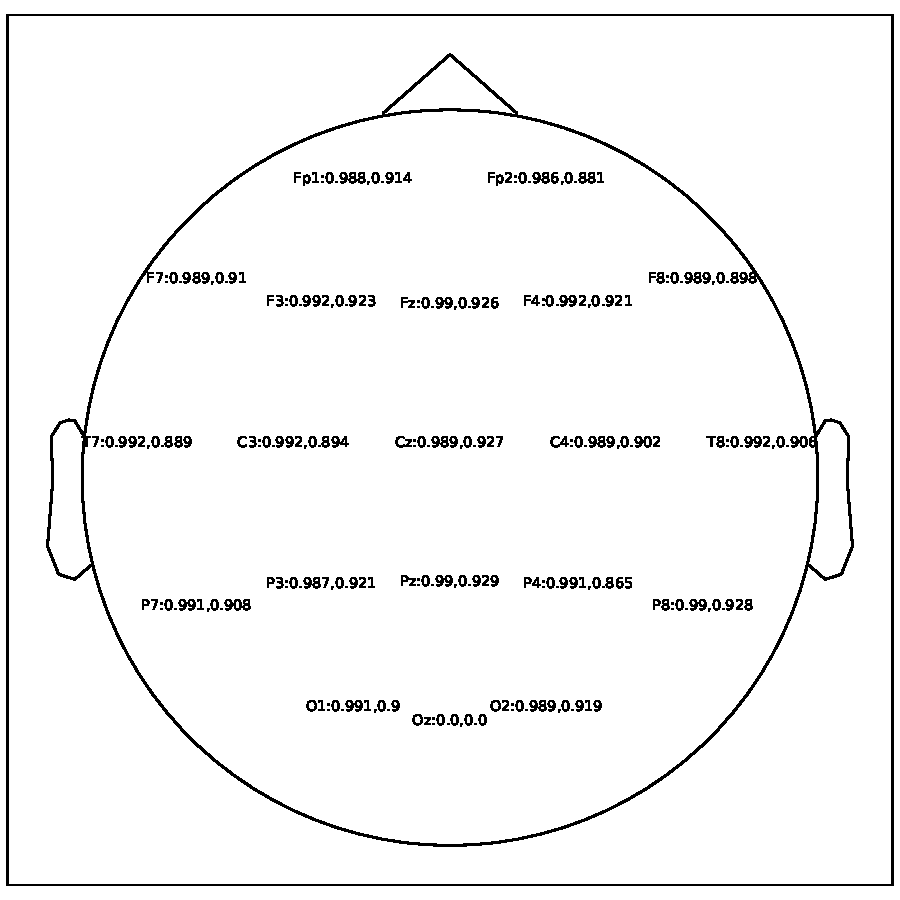
\includegraphics[width=.95\textwidth,trim={0cm 0cm 0cm 0cm},clip]{../SearchResults_2Ch/SearchSpaceResult_2Ch_(61)_S40_RemoveBaseLineOn_20191005}};
	  \begin{scope}[scale=1]
	      \draw[line width=2pt,blue] (-7.85,-7.85) node[anchor=west,right=.15cm] {\small{Best Channels according to the train accuracy}} circle (.2);
	      \draw[line width=2pt,red]  (7.85,-7.85)  node[anchor=east,left=.15cm] {\small{Best Channels according to the test accuracy}}  circle (.2);
	      %
	      %\draw[line width=2pt,blue] (-.2,-5.15) node[] (OzTr) {} circle (.45);
 	      %\draw[line width=2pt,blue] (1.65,-4.9) node[] (O2Tr) {} circle (.45);
 	      \draw[line width=2pt,blue] (-6.15,.15) node[] (T7Tr) {} circle (.45);
 	      %\draw[line width=2pt,blue] (-.2,.15) node[] (CzTr) {} circle (.4);
	      %\draw[line width=2pt,blue] (2.8,.15) node[] (C4Tr) {} circle (.4);
	      %\draw[line width=2pt,blue] (-.2,-5.15) node[] (OzTr) {} circle (.4);
 	      %\draw[line width=2pt,blue] (-2.05,-4.85) node[] (O1Tr) {} circle (.4);
 	      \draw[line width=2pt,blue] (5.75, .15) node[] (T8Tr) {} circle (.45);
	      %\draw[line width=2pt,blue] (4.6, 3.25) node[] (F8Tr) {} circle (.45);
	      \draw[line width=2pt,blue] (2.2, 2.85) node[] (F4Tr) {} circle (.45);
	      %\draw[line width=2pt,blue] (-5., -2.95) node[] (P7Tr) {} circle (.45);
	      %\draw[line width=2pt,blue] (4.6, -2.95) node[] (P8Tr) {} circle (.45);
	      %
	      %\draw[line width=2pt,red] (.6,2.8) node[] (FzTe) {} circle (.45);
	      %\draw[line width=2pt,red] (3.1, 2.85) node[] (F4Te) {} circle (.45);
	      %\draw[line width=2pt,red] (3.1,-2.5) node[] (P4Te) {} circle (.45);
	      \draw[line width=2pt,red] (.55,-2.5) node[] (PzTe) {} circle (.45);
	      \draw[line width=2pt,red] (5.4,-2.95) node[] (P8Te) {} circle (.45);
	      %\draw[line width=2pt,red] (5.45, 3.25) node[] (F8Te) {} circle (.45);
	      %\draw[line width=2pt,red] (-1.2, -4.85) node[] (O1Te) {} circle (.45);
	      %\draw[line width=2pt,red] (-2.3, .15) node[] (C3Te) {} circle (.45);
	      \draw[line width=2pt,red] (.65, .15) node[] (CzTe) {} circle (.45);
 	      %\draw[line width=2pt,red] (2.8+1, .15) node[] (C4Te) {} circle (.4);
 	      %\draw[line width=2pt,red] (6.65, .15) node[] (T8Te) {} circle (.4);
 	      %\draw[line width=2pt,red] (.7, -5.15) node[] (OzTe) {} circle (.45);
	\end{scope}
  \end{tikzpicture}
  \caption{Search for the second best channel with $40$ subjects, T10 is removed as baseline.}
  \label{fg:2Ch_S40_B1}
\end{figure}

%%%%%%%%%%%%%%%%%%%%%%%%%%%%%%%%%%%%%%%%%%%%%%%%%%%%%%%%%%%%%%%%%%%%%%%%%%%%%%%%%%%%%%%%%%%%%%%%%%%%%%%%%%%
% SearchSpaceResult_2Ch_(61)_S50_RemoveBaseLineOff_20191006
\newpage

\hspace*{12cm}\hyperlink{tab:TestResults}{(BACK TO RESULT TABLE)}

\bigskip
\bigskip

\begin{tabular}{ll}
  No. of Channels: & 2\\
  Previous Selected Channels: & Oz\\
  No. of Subjects: & 50\\
  Baseline Channel: & --\\
  Task:	& REO 
\end{tabular}

\bigskip

\begin{figure}[H]
  \tikzexternaldisable
  \centering
  \begin{tikzpicture}
	  \node[inner sep=0pt] (russell) at (0,0)
	      {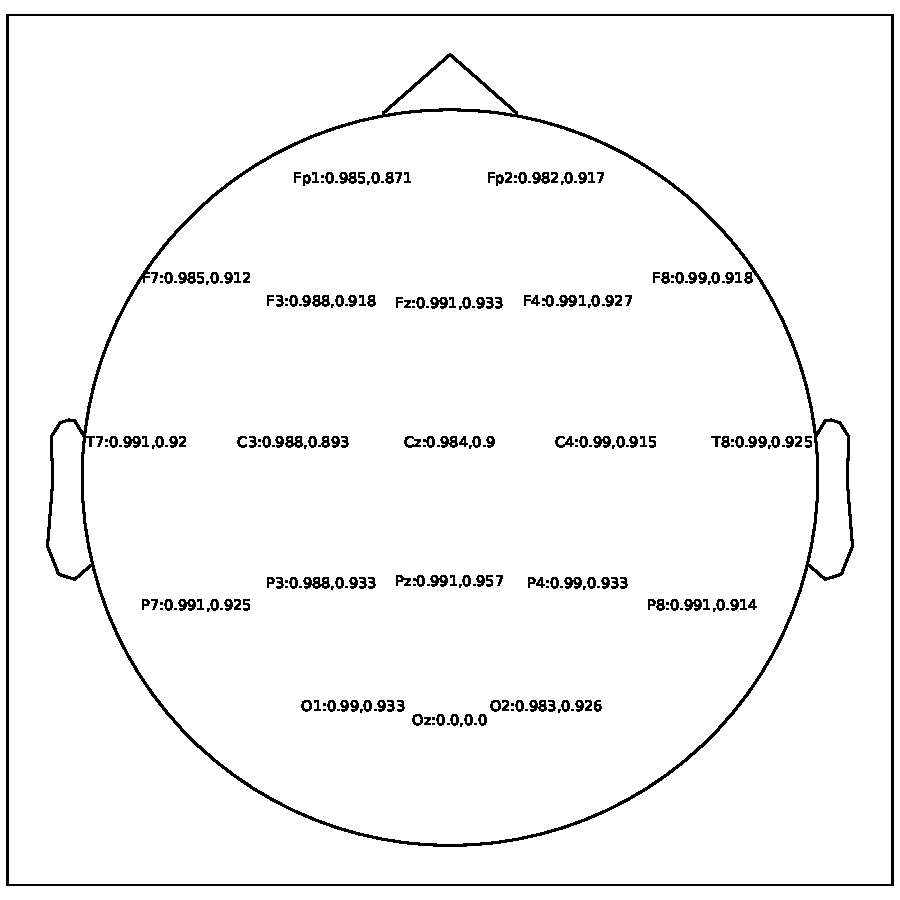
\includegraphics[width=.95\textwidth,trim={0cm 0cm 0cm 0cm},clip]{../SearchResults_2Ch/SearchSpaceResult_2Ch_(61)_S50_RemoveBaseLineOff_20191006}};
	  \begin{scope}[scale=1]
	      \draw[line width=2pt,blue] (-7.85,-7.85) node[anchor=west,right=.15cm] {\small{Best Channels according to the train accuracy}} circle (.2);
	      \draw[line width=2pt,red]  (7.85,-7.85)  node[anchor=east,left=.15cm] {\small{Best Channels according to the test accuracy}}  circle (.2);
	      %
	      %\draw[line width=2pt,blue] (-.2,-5.15) node[] (OzTr) {} circle (.45);
 	      %\draw[line width=2pt,blue] (1.65,-4.9) node[] (O2Tr) {} circle (.45);
 	      \draw[line width=2pt,blue] (-6.1,.15) node[] (T7Tr) {} circle (.45);
 	      %\draw[line width=2pt,blue] (-.2,.15) node[] (CzTr) {} circle (.4);
	      %\draw[line width=2pt,blue] (2.8,.15) node[] (C4Tr) {} circle (.4);
	      %\draw[line width=2pt,blue] (-.2,-5.15) node[] (OzTr) {} circle (.4);
 	      %\draw[line width=2pt,blue] (-2.05,-4.85) node[] (O1Tr) {} circle (.4);
 	      %\draw[line width=2pt,blue] (5.75, .15) node[] (T8Tr) {} circle (.45);
	      %\draw[line width=2pt,blue] (4.6, 3.25) node[] (F8Tr) {} circle (.45);
	      %\draw[line width=2pt,blue] (2.2, 2.85) node[] (F4Tr) {} circle (.45);
	      \draw[line width=2pt,blue] (-.25, 2.8) node[] (FzTr) {} circle (.45);
	      %\draw[line width=2pt,blue] (-5., -2.95) node[] (P7Tr) {} circle (.45);
	      %\draw[line width=2pt,blue] (4.6, -2.95) node[] (P8Tr) {} circle (.45);
		\draw[line width=2pt,blue] (-.25, -2.5) node[] (PzTr) {} circle (.45);
	      %
	      \draw[line width=2pt,red] (.6,2.8) node[] (FzTe) {} circle (.45);
	      %\draw[line width=2pt,red] (3.1, 2.85) node[] (F4Te) {} circle (.45);
	      %\draw[line width=2pt,red] (3.1,-2.5) node[] (P4Te) {} circle (.45);
	      \draw[line width=2pt,red] (.6,-2.5) node[] (PzTe) {} circle (.45);
	      %\draw[line width=2pt,red] (5.4,-2.95) node[] (P8Te) {} circle (.45);
	      %\draw[line width=2pt,red] (5.45, 3.25) node[] (F8Te) {} circle (.45);
	      \draw[line width=2pt,red] (-1.25, -4.85) node[] (O1Te) {} circle (.45);
	      %\draw[line width=2pt,red] (-2.3, .15) node[] (C3Te) {} circle (.45);
	      %\draw[line width=2pt,red] (.65, .15) node[] (CzTe) {} circle (.45);
 	      %\draw[line width=2pt,red] (2.8+1, .15) node[] (C4Te) {} circle (.4);
 	      %\draw[line width=2pt,red] (6.65, .15) node[] (T8Te) {} circle (.4);
 	      %\draw[line width=2pt,red] (.7, -5.15) node[] (OzTe) {} circle (.45);
	\end{scope}
  \end{tikzpicture}
  \caption{Search for the second best channel with $40$ subjects, no baseline is removed.}
  \label{fg:2Ch_S50_B0}
\end{figure}


%%%%%%%%%%%%%%%%%%%%%%%%%%%%%%%%%%%%%%%%%%%%%%%%%%%%%%%%%%%%%%%%%%%%%%%%%%%%%%%%%%%%%%%%%%%%%%%%%%%%%%%%%%%
% SearchSpaceResult_2Ch_(61)_S50_RemoveBaseLineOff_SamplesIn5Out20_20191015
\newpage

\global\pdfpageattr\expandafter{\the\pdfpageattr/Rotate 90}

\begin{landscape}
 


\hspace*{12cm}\hyperlink{tab:TestResults}{(BACK TO RESULT TABLE)}

Comparison of normal and reduced augmentation.

\begin{tabular}{ll}
  No. of Channels: & 2\\
  Previous Selected Channels: & Oz\\
  No. of Subjects: & 50\\
  Baseline Channel: & --\\
  In/Out Shift: & 4, 20\\
\end{tabular}

\begin{figure}[H]
  \tikzexternaldisable
  \centering
  \begin{tikzpicture}
	  \node[inner sep=0pt] (russell) at (12,0)
	      {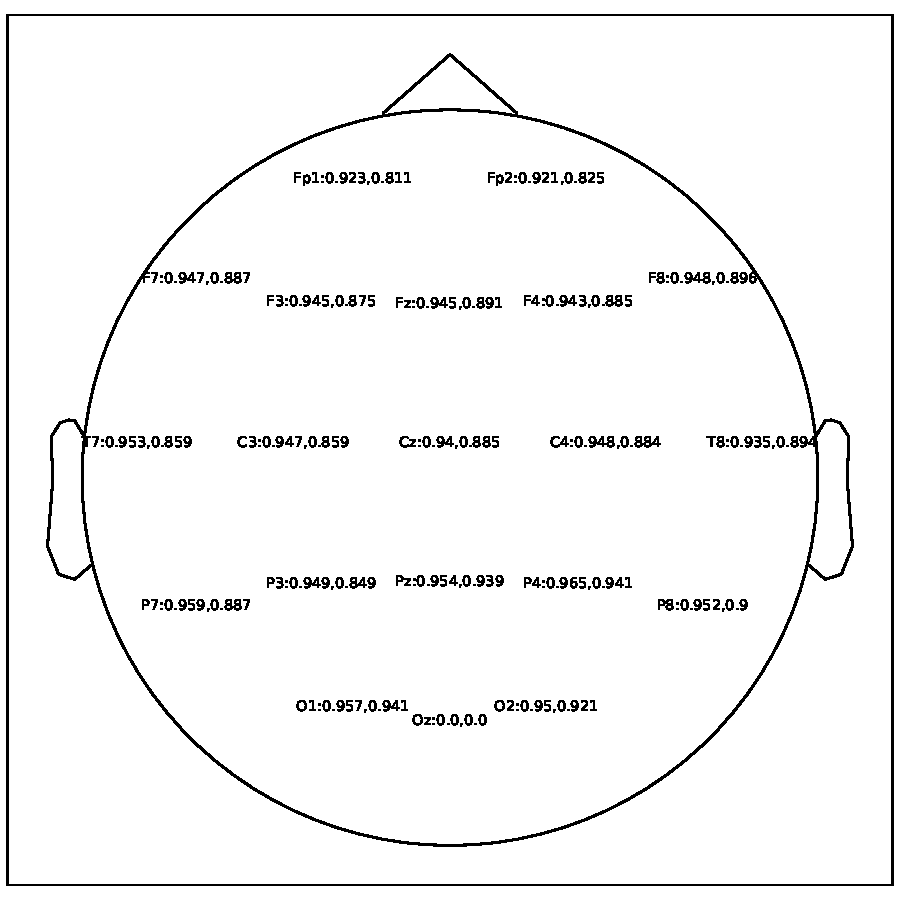
\includegraphics[width=.7\textwidth,trim={0cm 0cm 0cm 0cm},clip]{../SearchResults_2Ch/SearchSpaceResult_2Ch_(61)_S50_RemoveBaseLineOff_SamplesIn5Out20_20191015}};
 	  \node[inner sep=0pt] (russell) at (12,6.2) {Reduced Augmentation};
 	  \node[inner sep=0pt] (russell) at (0,0)
	      {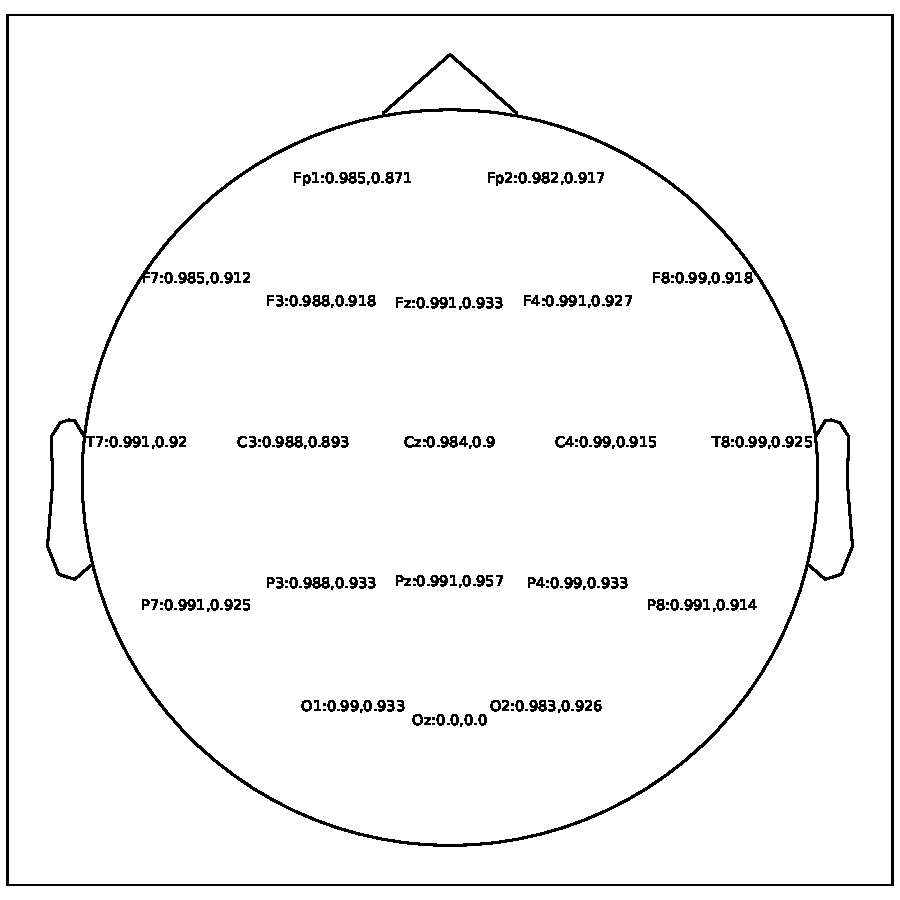
\includegraphics[width=.7\textwidth,trim={0cm 0cm 0cm 0cm},clip]{../SearchResults_2Ch/SearchSpaceResult_2Ch_(61)_S50_RemoveBaseLineOff_20191006}};
	  \node[inner sep=0pt] (russell) at (0,6.2) {Normal};
 	  
% 	  \begin{scope}[scale=1]
% 	      \draw[line width=2pt,blue] (-7.85,-7.85) node[anchor=west,right=.15cm] {\small{Best Channels according to the train accuracy}} circle (.2);
% 	      \draw[line width=2pt,red]  (7.85,-7.85)  node[anchor=east,left=.15cm] {\small{Best Channels according to the test accuracy}}  circle (.2);
% 	      %
% 	      %\draw[line width=2pt,blue] (-.2,-5.15) node[] (OzTr) {} circle (.45);
%  	      %\draw[line width=2pt,blue] (1.65,-4.9) node[] (O2Tr) {} circle (.45);
%  	      \draw[line width=2pt,blue] (-6.1,.15) node[] (T7Tr) {} circle (.45);
%  	      %\draw[line width=2pt,blue] (-.2,.15) node[] (CzTr) {} circle (.4);
% 	      %\draw[line width=2pt,blue] (2.8,.15) node[] (C4Tr) {} circle (.4);
% 	      %\draw[line width=2pt,blue] (-.2,-5.15) node[] (OzTr) {} circle (.4);
%  	      %\draw[line width=2pt,blue] (-2.05,-4.85) node[] (O1Tr) {} circle (.4);
%  	      %\draw[line width=2pt,blue] (5.75, .15) node[] (T8Tr) {} circle (.45);
% 	      %\draw[line width=2pt,blue] (4.6, 3.25) node[] (F8Tr) {} circle (.45);
% 	      %\draw[line width=2pt,blue] (2.2, 2.85) node[] (F4Tr) {} circle (.45);
% 	      \draw[line width=2pt,blue] (-.25, 2.8) node[] (FzTr) {} circle (.45);
% 	      %\draw[line width=2pt,blue] (-5., -2.95) node[] (P7Tr) {} circle (.45);
% 	      %\draw[line width=2pt,blue] (4.6, -2.95) node[] (P8Tr) {} circle (.45);
% 		\draw[line width=2pt,blue] (-.25, -2.5) node[] (PzTr) {} circle (.45);
% 	      %
% 	      \draw[line width=2pt,red] (.6,2.8) node[] (FzTe) {} circle (.45);
% 	      %\draw[line width=2pt,red] (3.1, 2.85) node[] (F4Te) {} circle (.45);
% 	      %\draw[line width=2pt,red] (3.1,-2.5) node[] (P4Te) {} circle (.45);
% 	      \draw[line width=2pt,red] (.6,-2.5) node[] (PzTe) {} circle (.45);
% 	      %\draw[line width=2pt,red] (5.4,-2.95) node[] (P8Te) {} circle (.45);
% 	      %\draw[line width=2pt,red] (5.45, 3.25) node[] (F8Te) {} circle (.45);
% 	      \draw[line width=2pt,red] (-1.25, -4.85) node[] (O1Te) {} circle (.45);
% 	      %\draw[line width=2pt,red] (-2.3, .15) node[] (C3Te) {} circle (.45);
% 	      %\draw[line width=2pt,red] (.65, .15) node[] (CzTe) {} circle (.45);
%  	      %\draw[line width=2pt,red] (2.8+1, .15) node[] (C4Te) {} circle (.4);
%  	      %\draw[line width=2pt,red] (6.65, .15) node[] (T8Te) {} circle (.4);
%  	      %\draw[line width=2pt,red] (.7, -5.15) node[] (OzTe) {} circle (.45);
% 	\end{scope}
  \end{tikzpicture}
  \caption{Comparison for the second best channel with $50$ subjects, no baseline is removed.}
  \label{fg:2Ch_S50_B0_RA}
\end{figure}

\end{landscape}



%%%%%%%%%%%%%%%%%%%%%%%%%%%%%%%%%%%%%%%%%%%%%%%%%%%%%%%%%%%%%%%%%%%%%%%%%%%%%%%%%%%%%%%%%%%%%%%%%%%%%%%%%%%
% SearchSpaceResult_2Ch_(61)_S50_RemoveBaseLineOn_20191011
\newpage

\global\pdfpageattr\expandafter{\the\pdfpageattr/Rotate 0}

\hspace*{12cm}\hyperlink{tab:TestResults}{(BACK TO RESULT TABLE)}

\bigskip
\bigskip

\begin{tabular}{ll}
  No. of Channels: & 2\\
  Previous Selected Channels: & Oz\\
  No. of Subjects: & 50\\
  Baseline Channel: & T10\\
  Task:	& REO 
\end{tabular}

\bigskip

\begin{figure}[H]
  \tikzexternaldisable
  \centering
  \begin{tikzpicture}
	  \node[inner sep=0pt] (russell) at (0,0)
	      {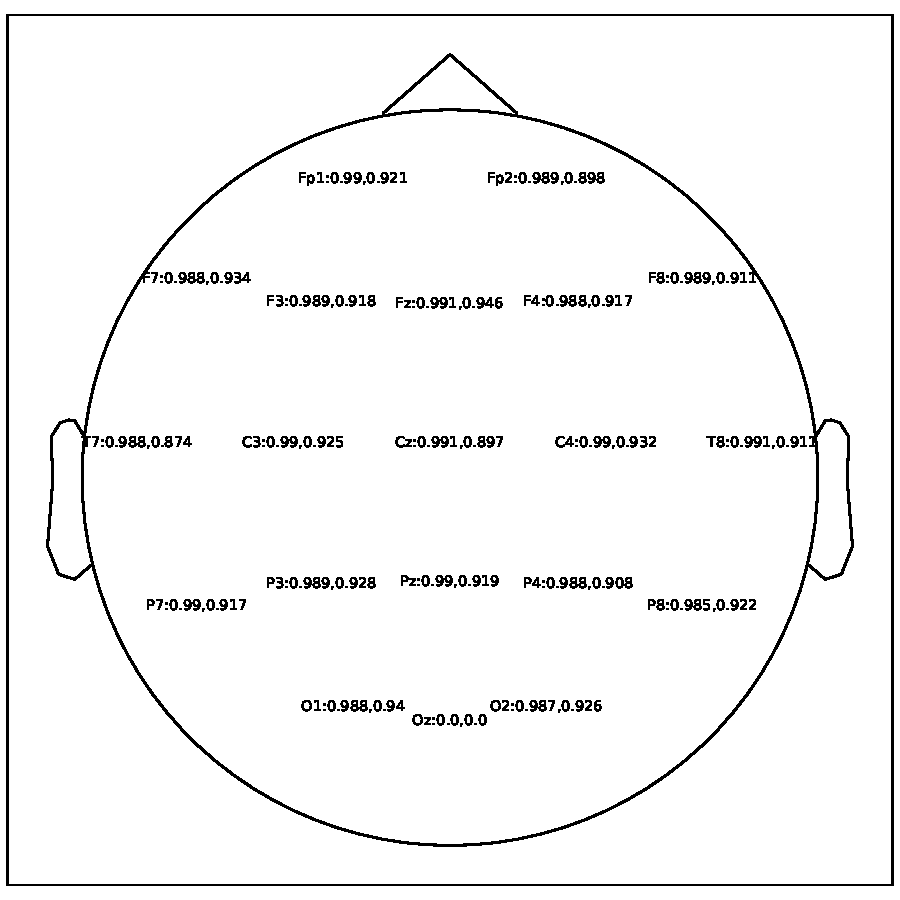
\includegraphics[width=.95\textwidth,trim={0cm 0cm 0cm 0cm},clip]{../SearchResults_2Ch/SearchSpaceResult_2Ch_(61)_S50_RemoveBaseLineOn_20191011}};
	  \begin{scope}[scale=1]
	      \draw[line width=2pt,blue] (-7.85,-7.85) node[anchor=west,right=.15cm] {\small{Best Channels according to the train accuracy}} circle (.2);
	      \draw[line width=2pt,red]  (7.85,-7.85)  node[anchor=east,left=.15cm] {\small{Best Channels according to the test accuracy}}  circle (.2);
	      %
	      %\draw[line width=2pt,blue] (-.2,-5.1) node[] (OzTr) {} circle (.45);
 	      %\draw[line width=2pt,blue] (1.65,-4.9) node[] (O2Tr) {} circle (.45);
 	      %\draw[line width=2pt,blue] (-6.1,.15) node[] (T7Tr) {} circle (.45);
	      \draw[line width=2pt,blue] (-.25,.15) node[] (CzTr) {} circle (.45);
	      %\draw[line width=2pt,blue] (2.75,.15) node[] (C4Tr) {} circle (.45);
	      %\draw[line width=2pt,blue] (-3.2,.15) node[] (C3Tr) {} circle (.45);
	      %\draw[line width=2pt,blue] (-2.05,-4.9) node[] (O1Tr) {} circle (.45);
 	      %\draw[line width=2pt,blue] (-2.05,-4.85) node[] (O1Tr) {} circle (.4);
 	      \draw[line width=2pt,blue] (5.75, .15) node[] (T8Tr) {} circle (.45);
	      %\draw[line width=2pt,blue] (4.6, 3.25) node[] (F8Tr) {} circle (.45);
	      %\draw[line width=2pt,blue] (2.2, 2.85) node[] (F4Tr) {} circle (.45);
	      \draw[line width=2pt,blue] (-.25, 2.8) node[] (FzTr) {} circle (.45);
	      %\draw[line width=2pt,blue] (-5., -2.95) node[] (P7Tr) {} circle (.45);
	      %\draw[line width=2pt,blue] (-2., 5.2) node[] (PF1Tr) {} circle (.45);
	      %\draw[line width=2pt,blue] (1.7, 5.2) node[] (PF2Tr) {} circle (.45);
	      %\draw[line width=2pt,blue] (4.6, -2.95) node[] (P8Tr) {} circle (.45);
	      %\draw[line width=2pt,blue] (-.25, -2.5) node[] (PzTr) {} circle (.45);
	      %
	      \draw[line width=2pt,red] (.6,2.8) node[] (FzTe) {} circle (.45);
	      %\draw[line width=2pt,red] (3.1, 2.85) node[] (F4Te) {} circle (.45);
	      %\draw[line width=2pt,red] (3.1,-2.5) node[] (P4Te) {} circle (.45);
	      %\draw[line width=2pt,red] (.6,-2.5) node[] (PzTe) {} circle (.45);
	      %\draw[line width=2pt,red] (5.45,-2.95) node[] (P8Te) {} circle (.45);
	      %\draw[line width=2pt,red] (2.55,5.2) node[] (FP2Te) {} circle (.45);
	      %\draw[line width=2pt,red] (5.45, 3.25) node[] (F8Te) {} circle (.45);
	      \draw[line width=2pt,red] (-4.15, 3.25) node[] (F7Te) {} circle (.45);
	      \draw[line width=2pt,red] (-1.25, -4.85) node[] (O1Te) {} circle (.45);
	      %\draw[line width=2pt,red] (-2.3, .15) node[] (C3Te) {} circle (.45);
	      %\draw[line width=2pt,red] (.65, .15) node[] (CzTe) {} circle (.45);
 	      %\draw[line width=2pt,red] (2.8+1, .15) node[] (C4Te) {} circle (.4);
	      %\draw[line width=2pt,red] (6.6, .15) node[] (T8Te) {} circle (.45);
 	      %\draw[line width=2pt,red] (.7, -5.1) node[] (OzTe) {} circle (.45);
	\end{scope}
  \end{tikzpicture}
  \caption{Search for the second best channel with $40$ subjects, T10 is removed as baseline.}
  \label{fg:2Ch_S50_B1}
\end{figure}


%%%%%%%%%%%%%%%%%%%%%%%%%%%%%%%%%%%%%%%%%%%%%%%%%%%%%%%%%%%%%%%%%%%%%%%%%%%%%%%%%%%%%%%%%%%%%%%%%%%%%%%%%%%
% SearchSpaceResult_2Ch_(61)_S50_RemoveBaseLineOn_SamplesIn5Out20_20191015
\newpage

\global\pdfpageattr\expandafter{\the\pdfpageattr/Rotate 90}

\begin{landscape}
 


\hspace*{12cm}\hyperlink{tab:TestResults}{(BACK TO RESULT TABLE)}

Comparison of normal and reduced augmentation.

\begin{tabular}{ll}
  No. of Channels: & 2\\
  Previous Selected Channels: & Oz\\
  No. of Subjects: & 50\\
  Baseline Channel: & T10\\
  In/Out Shift: & 4, 20\\
\end{tabular}

\begin{figure}[H]
  \tikzexternaldisable
  \centering
  \begin{tikzpicture}
	  \node[inner sep=0pt] (russell) at (12,0)
	      {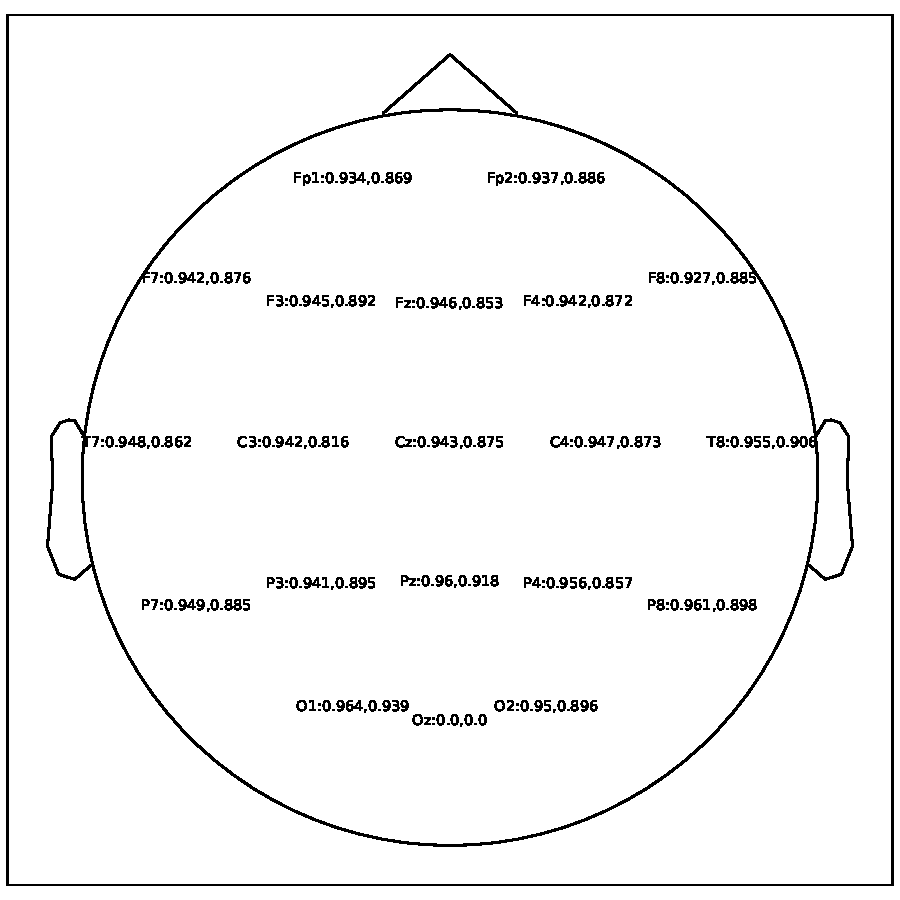
\includegraphics[width=.65\textwidth,trim={0cm 0cm 0cm 0cm},clip]{../SearchResults_2Ch/SearchSpaceResult_2Ch_(61)_S50_RemoveBaseLineOn_SamplesIn5Out20_20191015}};
 	  \node[inner sep=0pt] (russell) at (12,6.15) {Reduced Augmentation};
 	  \node[inner sep=0pt] (russell) at (0,0)
	      {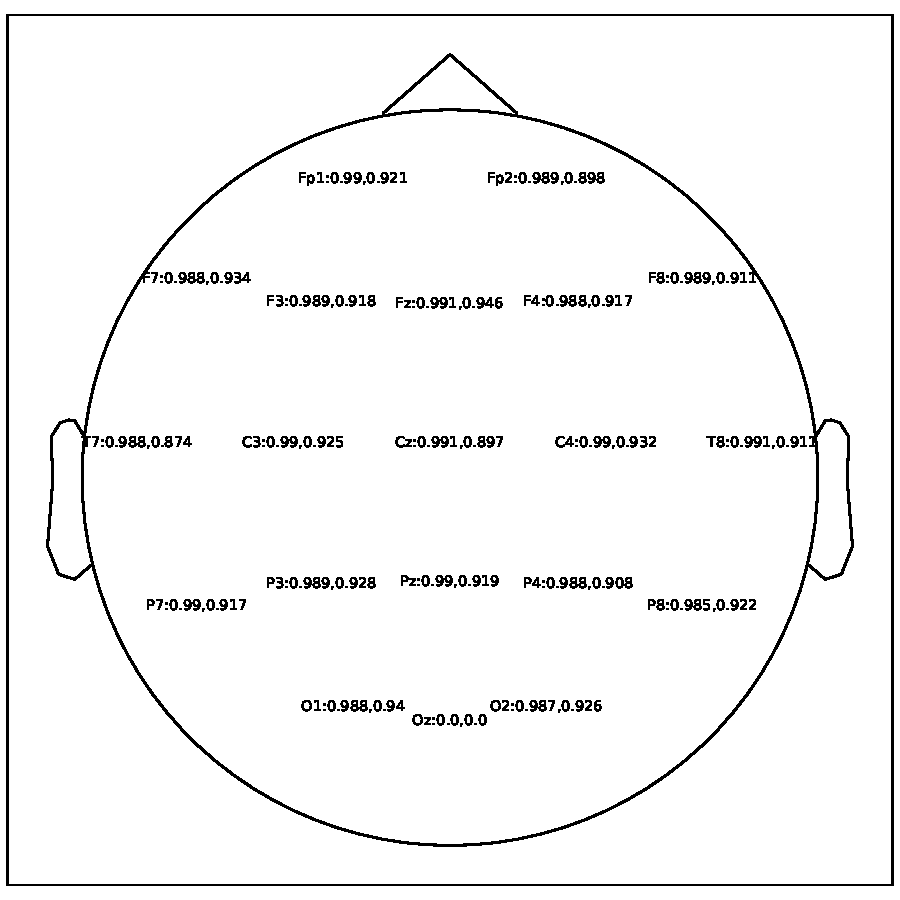
\includegraphics[width=.65\textwidth,trim={0cm 0cm 0cm 0cm},clip]{../SearchResults_2Ch/SearchSpaceResult_2Ch_(61)_S50_RemoveBaseLineOn_20191011}};
	  \node[inner sep=0pt] (russell) at (0,6.15) {Normal};
 	  
% 	  \begin{scope}[scale=1]
% 	      \draw[line width=2pt,blue] (-7.85,-7.85) node[anchor=west,right=.15cm] {\small{Best Channels according to the train accuracy}} circle (.2);
% 	      \draw[line width=2pt,red]  (7.85,-7.85)  node[anchor=east,left=.15cm] {\small{Best Channels according to the test accuracy}}  circle (.2);
% 	      %
% 	      %\draw[line width=2pt,blue] (-.2,-5.15) node[] (OzTr) {} circle (.45);
%  	      %\draw[line width=2pt,blue] (1.65,-4.9) node[] (O2Tr) {} circle (.45);
%  	      \draw[line width=2pt,blue] (-6.1,.15) node[] (T7Tr) {} circle (.45);
%  	      %\draw[line width=2pt,blue] (-.2,.15) node[] (CzTr) {} circle (.4);
% 	      %\draw[line width=2pt,blue] (2.8,.15) node[] (C4Tr) {} circle (.4);
% 	      %\draw[line width=2pt,blue] (-.2,-5.15) node[] (OzTr) {} circle (.4);
%  	      %\draw[line width=2pt,blue] (-2.05,-4.85) node[] (O1Tr) {} circle (.4);
%  	      %\draw[line width=2pt,blue] (5.75, .15) node[] (T8Tr) {} circle (.45);
% 	      %\draw[line width=2pt,blue] (4.6, 3.25) node[] (F8Tr) {} circle (.45);
% 	      %\draw[line width=2pt,blue] (2.2, 2.85) node[] (F4Tr) {} circle (.45);
% 	      \draw[line width=2pt,blue] (-.25, 2.8) node[] (FzTr) {} circle (.45);
% 	      %\draw[line width=2pt,blue] (-5., -2.95) node[] (P7Tr) {} circle (.45);
% 	      %\draw[line width=2pt,blue] (4.6, -2.95) node[] (P8Tr) {} circle (.45);
% 		\draw[line width=2pt,blue] (-.25, -2.5) node[] (PzTr) {} circle (.45);
% 	      %
% 	      \draw[line width=2pt,red] (.6,2.8) node[] (FzTe) {} circle (.45);
% 	      %\draw[line width=2pt,red] (3.1, 2.85) node[] (F4Te) {} circle (.45);
% 	      %\draw[line width=2pt,red] (3.1,-2.5) node[] (P4Te) {} circle (.45);
% 	      \draw[line width=2pt,red] (.6,-2.5) node[] (PzTe) {} circle (.45);
% 	      %\draw[line width=2pt,red] (5.4,-2.95) node[] (P8Te) {} circle (.45);
% 	      %\draw[line width=2pt,red] (5.45, 3.25) node[] (F8Te) {} circle (.45);
% 	      \draw[line width=2pt,red] (-1.25, -4.85) node[] (O1Te) {} circle (.45);
% 	      %\draw[line width=2pt,red] (-2.3, .15) node[] (C3Te) {} circle (.45);
% 	      %\draw[line width=2pt,red] (.65, .15) node[] (CzTe) {} circle (.45);
%  	      %\draw[line width=2pt,red] (2.8+1, .15) node[] (C4Te) {} circle (.4);
%  	      %\draw[line width=2pt,red] (6.65, .15) node[] (T8Te) {} circle (.4);
%  	      %\draw[line width=2pt,red] (.7, -5.15) node[] (OzTe) {} circle (.45);
% 	\end{scope}
  \end{tikzpicture}
  \caption{Comparison for the second best channel with $50$ subjects, T10 is removed as baseline.}
  \label{fg:2Ch_S50_B1_RA}
\end{figure}

\end{landscape}

\global\pdfpageattr\expandafter{\the\pdfpageattr/Rotate -90}


%%%%%%%%%%%%%%%%%%%%%%%%%%%%%%%%%%%%%%%%%%%%%%%%%%%%%%%%%%%%%%%%%%%%%%%%%%%%%%%%%%%%%%%%%%%%%%%%%%%%%%%%%%%
% SearchSpaceResult_3Ch_(61_35)_S30_RemoveBaseLineOff_20191005
\newpage

\global\pdfpageattr\expandafter{\the\pdfpageattr/Rotate 0}

\hspace*{12cm}\hyperlink{tab:TestResults}{(BACK TO RESULT TABLE)}

\bigskip
\bigskip

\begin{tabular}{ll}
  No. of Channels: & 3\\
  Previous Selected Channels: & Oz, F4\\
  No. of Subjects: & 30\\
  Baseline Channel: & --\\
  Task:	& REO 
\end{tabular}

\bigskip

\begin{figure}[H]
  \tikzexternaldisable
  \centering
  \begin{tikzpicture}
	  \node[inner sep=0pt] (russell) at (0,0)
	      {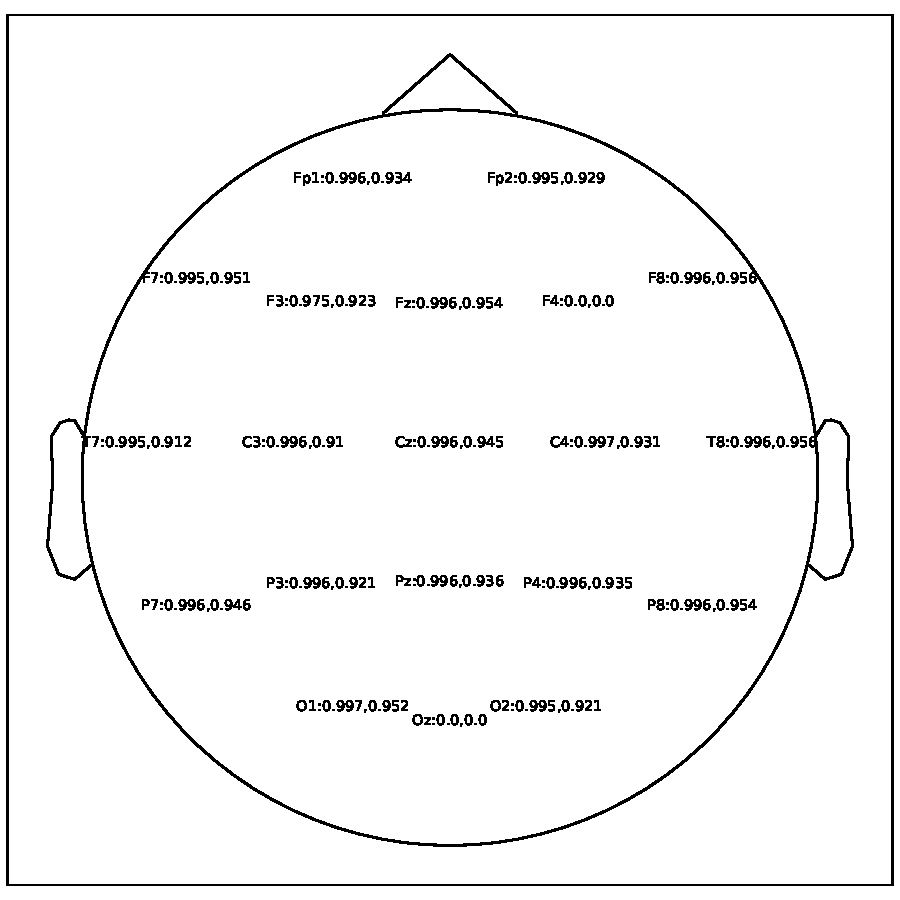
\includegraphics[width=.95\textwidth,trim={0cm 0cm 0cm 0cm},clip]{../SearchResults_3Ch/SearchSpaceResult_3Ch_(61_35)_S30_RemoveBaseLineOff_20191005}};
	  \begin{scope}[scale=1]
	      \draw[line width=2pt,blue] (-7.85,-7.85) node[anchor=west,right=.15cm] {\small{Best Channels according to the train accuracy}} circle (.2);
	      \draw[line width=2pt,red]  (7.85,-7.85)  node[anchor=east,left=.15cm] {\small{Best Channels according to the test accuracy}}  circle (.2);
	      %
	      %\draw[line width=2pt,blue] (-.2,-5.1) node[] (OzTr) {} circle (.45);
 	      %\draw[line width=2pt,blue] (1.65,-4.9) node[] (O2Tr) {} circle (.45);
 	      %\draw[line width=2pt,blue] (-6.1,.15) node[] (T7Tr) {} circle (.45);
	      \draw[line width=2pt,blue] (-.25,.15) node[] (CzTr) {} circle (.45);
	      \draw[line width=2pt,blue] (2.75,.15) node[] (C4Tr) {} circle (.45);
	      \draw[line width=2pt,blue] (-2.05,-4.9) node[] (O1Tr) {} circle (.45);
 	      %\draw[line width=2pt,blue] (-2.05,-4.85) node[] (O1Tr) {} circle (.4);
 	      %\draw[line width=2pt,blue] (5.75, .15) node[] (T8Tr) {} circle (.45);
	      %\draw[line width=2pt,blue] (4.6, 3.25) node[] (F8Tr) {} circle (.45);
	      %\draw[line width=2pt,blue] (2.2, 2.85) node[] (F4Tr) {} circle (.45);
	      %\draw[line width=2pt,blue] (-.25, 2.8) node[] (FzTr) {} circle (.45);
	      %\draw[line width=2pt,blue] (-5., -2.95) node[] (P7Tr) {} circle (.45);
	      %\draw[line width=2pt,blue] (4.6, -2.95) node[] (P8Tr) {} circle (.45);
	      %\draw[line width=2pt,blue] (-.25, -2.5) node[] (PzTr) {} circle (.45);
	      %
	      \draw[line width=2pt,red] (.6,2.8) node[] (FzTe) {} circle (.45);
	      %\draw[line width=2pt,red] (3.1, 2.85) node[] (F4Te) {} circle (.45);
	      %\draw[line width=2pt,red] (3.1,-2.5) node[] (P4Te) {} circle (.45);
	      %\draw[line width=2pt,red] (.6,-2.5) node[] (PzTe) {} circle (.45);
	      %\draw[line width=2pt,red] (5.4,-2.95) node[] (P8Te) {} circle (.45);
	      \draw[line width=2pt,red] (5.45, 3.25) node[] (F8Te) {} circle (.45);
	      %\draw[line width=2pt,red] (-1.25, -4.85) node[] (O1Te) {} circle (.45);
	      %\draw[line width=2pt,red] (-2.3, .15) node[] (C3Te) {} circle (.45);
	      %\draw[line width=2pt,red] (.65, .15) node[] (CzTe) {} circle (.45);
 	      %\draw[line width=2pt,red] (2.8+1, .15) node[] (C4Te) {} circle (.4);
	      \draw[line width=2pt,red] (6.6, .15) node[] (T8Te) {} circle (.45);
 	      %\draw[line width=2pt,red] (.7, -5.1) node[] (OzTe) {} circle (.45);
	\end{scope}
  \end{tikzpicture}
  \caption{Search for the third best channel with $30$ subjects, no baseline is removed.}
  \label{fg:3Ch_S30_B0}
\end{figure}


%%%%%%%%%%%%%%%%%%%%%%%%%%%%%%%%%%%%%%%%%%%%%%%%%%%%%%%%%%%%%%%%%%%%%%%%%%%%%%%%%%%%%%%%%%%%%%%%%%%%%%%%%%%
% SearchSpaceResult_3Ch_(61_35)_S30_RemoveBaseLineOn_20191011
\newpage

\hspace*{12cm}\hyperlink{tab:TestResults}{(BACK TO RESULT TABLE)}

\bigskip
\bigskip

\begin{tabular}{ll}
  No. of Channels: & 3\\
  Previous Selected Channels: & Oz, F4\\
  No. of Subjects: & 30\\
  Baseline Channel: & T10\\
  Task:	& REO 
\end{tabular}

\bigskip

\begin{figure}[H]
  \tikzexternaldisable
  \centering
  \begin{tikzpicture}
	  \node[inner sep=0pt] (russell) at (0,0)
	      {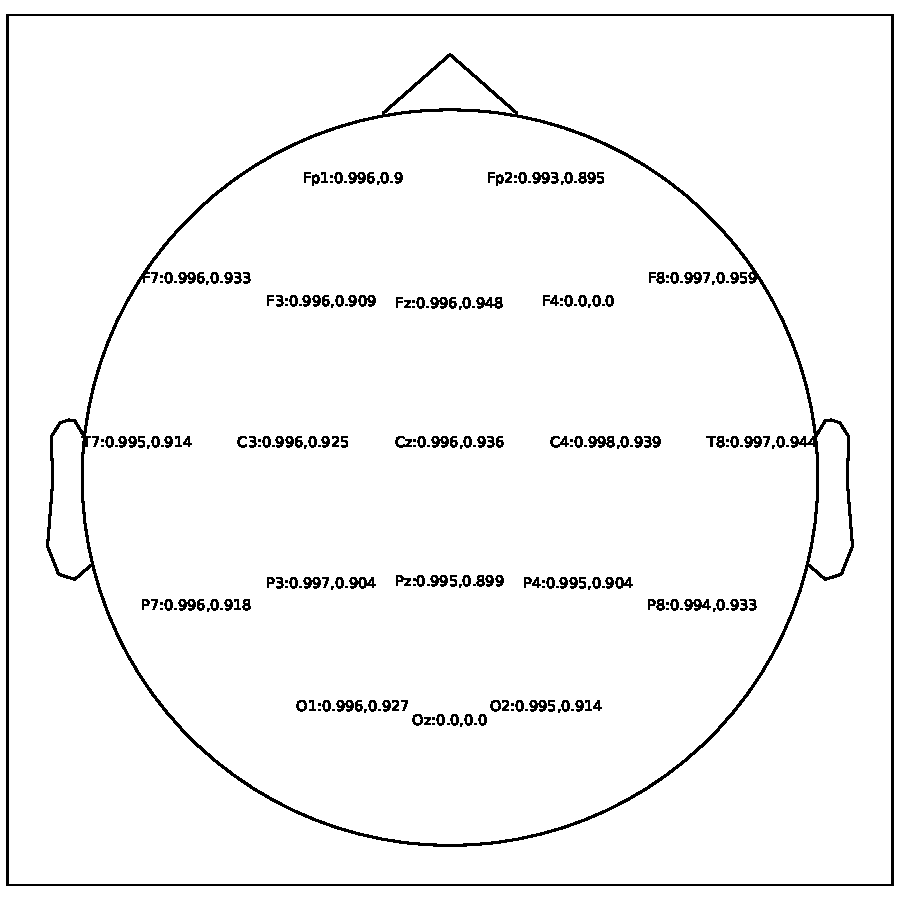
\includegraphics[width=.95\textwidth,trim={0cm 0cm 0cm 0cm},clip]{../SearchResults_3Ch/SearchSpaceResult_3Ch_(61_35)_S30_RemoveBaseLineOn_20191011}};
	  \begin{scope}[scale=1]
	      \draw[line width=2pt,blue] (-7.85,-7.85) node[anchor=west,right=.15cm] {\small{Best Channels according to the train accuracy}} circle (.2);
	      \draw[line width=2pt,red]  (7.85,-7.85)  node[anchor=east,left=.15cm] {\small{Best Channels according to the test accuracy}}  circle (.2);
	      %
	      %\draw[line width=2pt,blue] (-.2,-5.1) node[] (OzTr) {} circle (.45);
 	      %\draw[line width=2pt,blue] (1.65,-4.9) node[] (O2Tr) {} circle (.45);
 	      %\draw[line width=2pt,blue] (-6.1,.15) node[] (T7Tr) {} circle (.45);
	      %\draw[line width=2pt,blue] (-.25,.15) node[] (CzTr) {} circle (.45);
	      \draw[line width=2pt,blue] (2.75,.15) node[] (C4Tr) {} circle (.45);
	      %\draw[line width=2pt,blue] (-3.2,.15) node[] (C3Tr) {} circle (.45);
	      %\draw[line width=2pt,blue] (-2.05,-4.9) node[] (O1Tr) {} circle (.45);
 	      %\draw[line width=2pt,blue] (-2.05,-4.85) node[] (O1Tr) {} circle (.4);
 	      %\draw[line width=2pt,blue] (5.75, .15) node[] (T8Tr) {} circle (.45);
	      \draw[line width=2pt,blue] (4.6, 3.25) node[] (F8Tr) {} circle (.45);
	      %\draw[line width=2pt,blue] (2.2, 2.85) node[] (F4Tr) {} circle (.45);
	      %\draw[line width=2pt,blue] (-.25, 2.8) node[] (FzTr) {} circle (.45);
	      %\draw[line width=2pt,blue] (-5., -2.95) node[] (P7Tr) {} circle (.45);
	      %\draw[line width=2pt,blue] (-2., 5.2) node[] (PF1Tr) {} circle (.45);
	      %\draw[line width=2pt,blue] (1.7, 5.2) node[] (PF2Tr) {} circle (.45);
	      %\draw[line width=2pt,blue] (4.6, -2.95) node[] (P8Tr) {} circle (.45);
		\draw[line width=2pt,blue] (-2.7, -2.5) node[] (P3Tr) {} circle (.45);
	      %\draw[line width=2pt,blue] (-.25, -2.5) node[] (PzTr) {} circle (.45);
	      %
	      \draw[line width=2pt,red] (.6,2.8) node[] (FzTe) {} circle (.45);
	      %\draw[line width=2pt,red] (3.1, 2.85) node[] (F4Te) {} circle (.45);
	      %\draw[line width=2pt,red] (3.1,-2.5) node[] (P4Te) {} circle (.45);
	      %\draw[line width=2pt,red] (.6,-2.5) node[] (PzTe) {} circle (.45);
	      %\draw[line width=2pt,red] (5.45,-2.95) node[] (P8Te) {} circle (.45);
	      %\draw[line width=2pt,red] (2.55,5.2) node[] (FP2Te) {} circle (.45);
	      \draw[line width=2pt,red] (5.45, 3.25) node[] (F8Te) {} circle (.45);
	      %\draw[line width=2pt,red] (-4.15, 3.25) node[] (F7Te) {} circle (.45);
	      %\draw[line width=2pt,red] (-1.25, -4.85) node[] (O1Te) {} circle (.45);
	      %\draw[line width=2pt,red] (-2.3, .15) node[] (C3Te) {} circle (.45);
	      %\draw[line width=2pt,red] (.65, .15) node[] (CzTe) {} circle (.45);
 	      %\draw[line width=2pt,red] (2.8+1, .15) node[] (C4Te) {} circle (.4);
	      \draw[line width=2pt,red] (6.6, .15) node[] (T8Te) {} circle (.45);
 	      %\draw[line width=2pt,red] (.7, -5.1) node[] (OzTe) {} circle (.45);
	\end{scope}
  \end{tikzpicture}
  \caption{Search for the third best channel with $30$ subjects, T10 is removed as baseline.}
  \label{fg:3Ch_S30_B1}
\end{figure}



%%%%%%%%%%%%%%%%%%%%%%%%%%%%%%%%%%%%%%%%%%%%%%%%%%%%%%%%%%%%%%%%%%%%%%%%%%%%%%%%%%%%%%%%%%%%%%%%%%%%%%%%%%%
% SearchSpaceResult_3Ch_(61_35)_S40_RemoveBaseLineOff_20191006
\newpage

\hspace*{12cm}\hyperlink{tab:TestResults}{(BACK TO RESULT TABLE)}

\bigskip
\bigskip

\begin{tabular}{ll}
  No. of Channels: & 3\\
  Previous Selected Channels: & Oz, F4\\
  No. of Subjects: & 40\\
  Baseline Channel: & --\\
  Task:	& REO 
\end{tabular}

\bigskip

\begin{figure}[H]
  \tikzexternaldisable
  \centering
  \begin{tikzpicture}
	  \node[inner sep=0pt] (russell) at (0,0)
	      {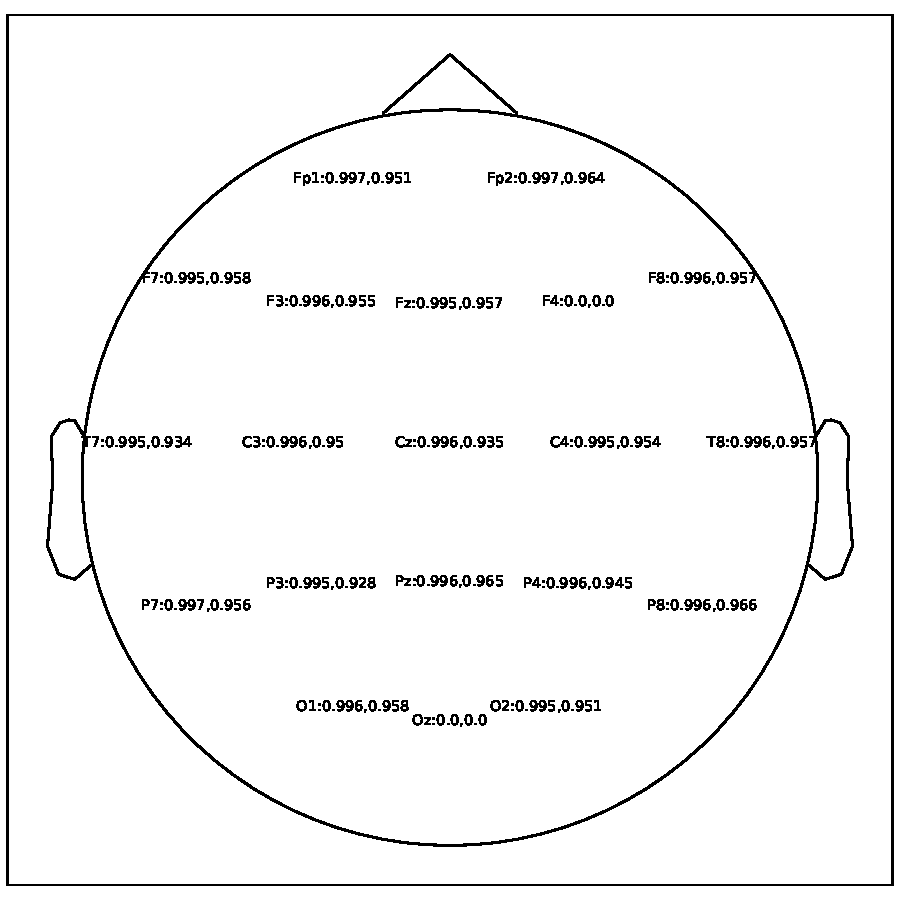
\includegraphics[width=.95\textwidth,trim={0cm 0cm 0cm 0cm},clip]{../SearchResults_3Ch/SearchSpaceResult_3Ch_(61_35)_S40_RemoveBaseLineOff_20191006}};
	  \begin{scope}[scale=1]
	      \draw[line width=2pt,blue] (-7.85,-7.85) node[anchor=west,right=.15cm] {\small{Best Channels according to the train accuracy}} circle (.2);
	      \draw[line width=2pt,red]  (7.85,-7.85)  node[anchor=east,left=.15cm] {\small{Best Channels according to the test accuracy}}  circle (.2);
	      %
	      %\draw[line width=2pt,blue] (-.2,-5.1) node[] (OzTr) {} circle (.45);
 	      %\draw[line width=2pt,blue] (1.65,-4.9) node[] (O2Tr) {} circle (.45);
 	      %\draw[line width=2pt,blue] (-6.1,.15) node[] (T7Tr) {} circle (.45);
	      %\draw[line width=2pt,blue] (-.25,.15) node[] (CzTr) {} circle (.45);
	      %\draw[line width=2pt,blue] (2.75,.15) node[] (C4Tr) {} circle (.45);
	      %\draw[line width=2pt,blue] (-2.05,-4.9) node[] (O1Tr) {} circle (.45);
 	      %\draw[line width=2pt,blue] (-2.05,-4.85) node[] (O1Tr) {} circle (.4);
 	      %\draw[line width=2pt,blue] (5.75, .15) node[] (T8Tr) {} circle (.45);
	      %\draw[line width=2pt,blue] (4.6, 3.25) node[] (F8Tr) {} circle (.45);
	      %\draw[line width=2pt,blue] (2.2, 2.85) node[] (F4Tr) {} circle (.45);
	      %\draw[line width=2pt,blue] (-.25, 2.8) node[] (FzTr) {} circle (.45);
	      \draw[line width=2pt,blue] (-5., -2.95) node[] (P7Tr) {} circle (.45);
	      \draw[line width=2pt,blue] (-2., 5.2) node[] (PF1Tr) {} circle (.45);
	      \draw[line width=2pt,blue] (1.7, 5.2) node[] (PF2Tr) {} circle (.45);
	      %\draw[line width=2pt,blue] (4.6, -2.95) node[] (P8Tr) {} circle (.45);
	      %\draw[line width=2pt,blue] (-.25, -2.5) node[] (PzTr) {} circle (.45);
	      %
	      %\draw[line width=2pt,red] (.6,2.8) node[] (FzTe) {} circle (.45);
	      %\draw[line width=2pt,red] (3.1, 2.85) node[] (F4Te) {} circle (.45);
	      %\draw[line width=2pt,red] (3.1,-2.5) node[] (P4Te) {} circle (.45);
	      \draw[line width=2pt,red] (.6,-2.5) node[] (PzTe) {} circle (.45);
	      \draw[line width=2pt,red] (5.45,-2.95) node[] (P8Te) {} circle (.45);
	      \draw[line width=2pt,red] (2.55,5.2) node[] (FP2Te) {} circle (.45);
	      %\draw[line width=2pt,red] (5.45, 3.25) node[] (F8Te) {} circle (.45);
	      %\draw[line width=2pt,red] (-1.25, -4.85) node[] (O1Te) {} circle (.45);
	      %\draw[line width=2pt,red] (-2.3, .15) node[] (C3Te) {} circle (.45);
	      %\draw[line width=2pt,red] (.65, .15) node[] (CzTe) {} circle (.45);
 	      %\draw[line width=2pt,red] (2.8+1, .15) node[] (C4Te) {} circle (.4);
	      %\draw[line width=2pt,red] (6.6, .15) node[] (T8Te) {} circle (.45);
 	      %\draw[line width=2pt,red] (.7, -5.1) node[] (OzTe) {} circle (.45);
	\end{scope}
  \end{tikzpicture}
  \caption{Search for the third best channel with $40$ subjects, no baseline is removed.}
  \label{fg:3Ch_S40_B0}
\end{figure}


%%%%%%%%%%%%%%%%%%%%%%%%%%%%%%%%%%%%%%%%%%%%%%%%%%%%%%%%%%%%%%%%%%%%%%%%%%%%%%%%%%%%%%%%%%%%%%%%%%%%%%%%%%%
% SearchSpaceResult_3Ch_(61_35)_S40_RemoveBaseLineOn_20191006
\newpage

\hspace*{12cm}\hyperlink{tab:TestResults}{(BACK TO RESULT TABLE)}

\bigskip
\bigskip

\begin{tabular}{ll}
  No. of Channels: & 3\\
  Previous Selected Channels: & Oz, F4\\
  No. of Subjects: & 40\\
  Baseline Channel: & T10\\
  Task:	& REO 
\end{tabular}

\bigskip

\begin{figure}[H]
  \tikzexternaldisable
  \centering
  \begin{tikzpicture}
	  \node[inner sep=0pt] (russell) at (0,0)
	      {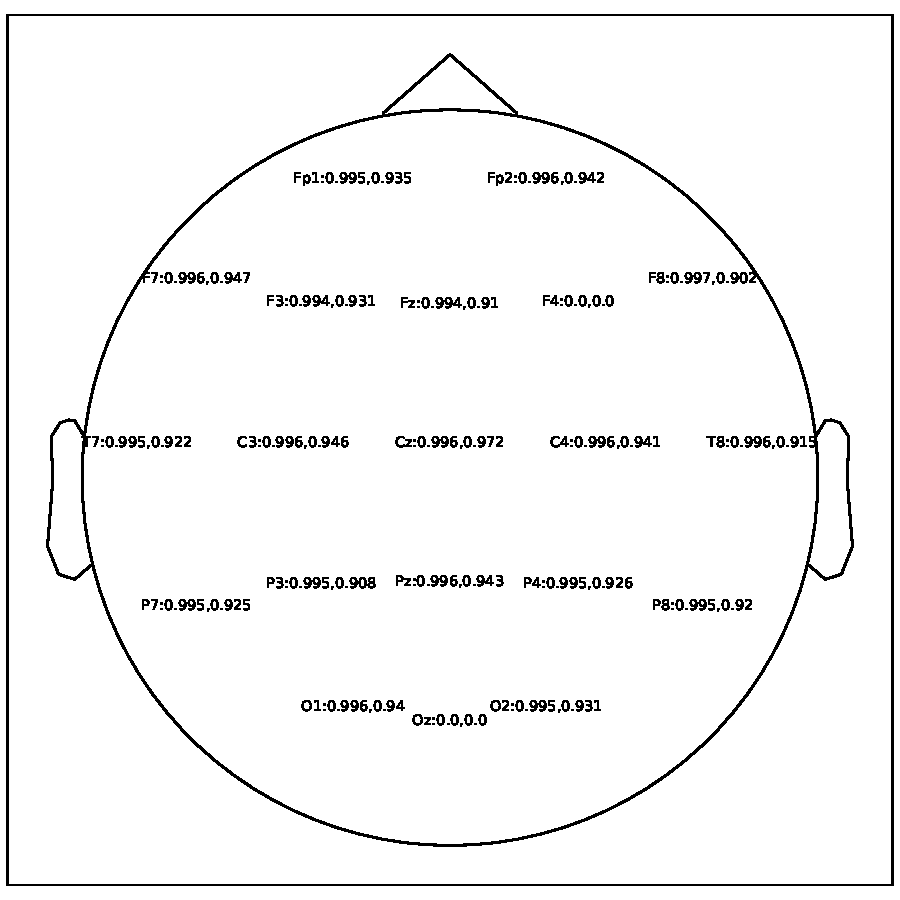
\includegraphics[width=.95\textwidth,trim={0cm 0cm 0cm 0cm},clip]{../SearchResults_3Ch/SearchSpaceResult_3Ch_(61_35)_S40_RemoveBaseLineOn_20191006}};
	  \begin{scope}[scale=1]
	      \draw[line width=2pt,blue] (-7.85,-7.85) node[anchor=west,right=.15cm] {\small{Best Channels according to the train accuracy}} circle (.2);
	      \draw[line width=2pt,red]  (7.85,-7.85)  node[anchor=east,left=.15cm] {\small{Best Channels according to the test accuracy}}  circle (.2);
	      %
	      %\draw[line width=2pt,blue] (-.2,-5.1) node[] (OzTr) {} circle (.45);
 	      %\draw[line width=2pt,blue] (1.65,-4.9) node[] (O2Tr) {} circle (.45);
 	      %\draw[line width=2pt,blue] (-6.1,.15) node[] (T7Tr) {} circle (.45);
	      %\draw[line width=2pt,blue] (-.25,.15) node[] (CzTr) {} circle (.45);
	      \draw[line width=2pt,blue] (2.75,.15) node[] (C4Tr) {} circle (.45);
	      \draw[line width=2pt,blue] (-3.2,.15) node[] (C3Tr) {} circle (.45);
	      %\draw[line width=2pt,blue] (-2.05,-4.9) node[] (O1Tr) {} circle (.45);
 	      %\draw[line width=2pt,blue] (-2.05,-4.85) node[] (O1Tr) {} circle (.4);
 	      %\draw[line width=2pt,blue] (5.75, .15) node[] (T8Tr) {} circle (.45);
	      \draw[line width=2pt,blue] (4.6, 3.25) node[] (F8Tr) {} circle (.45);
	      %\draw[line width=2pt,blue] (2.2, 2.85) node[] (F4Tr) {} circle (.45);
	      %\draw[line width=2pt,blue] (-.25, 2.8) node[] (FzTr) {} circle (.45);
	      %\draw[line width=2pt,blue] (-5., -2.95) node[] (P7Tr) {} circle (.45);
	      %\draw[line width=2pt,blue] (-2., 5.2) node[] (PF1Tr) {} circle (.45);
	      %\draw[line width=2pt,blue] (1.7, 5.2) node[] (PF2Tr) {} circle (.45);
	      %\draw[line width=2pt,blue] (4.6, -2.95) node[] (P8Tr) {} circle (.45);
	      %\draw[line width=2pt,blue] (-.25, -2.5) node[] (PzTr) {} circle (.45);
	      %
	      %\draw[line width=2pt,red] (.6,2.8) node[] (FzTe) {} circle (.45);
	      %\draw[line width=2pt,red] (3.1, 2.85) node[] (F4Te) {} circle (.45);
	      %\draw[line width=2pt,red] (3.1,-2.5) node[] (P4Te) {} circle (.45);
	      %\draw[line width=2pt,red] (.6,-2.5) node[] (PzTe) {} circle (.45);
	      %\draw[line width=2pt,red] (5.45,-2.95) node[] (P8Te) {} circle (.45);
	      %\draw[line width=2pt,red] (2.55,5.2) node[] (FP2Te) {} circle (.45);
	      %\draw[line width=2pt,red] (5.45, 3.25) node[] (F8Te) {} circle (.45);
	      \draw[line width=2pt,red] (-4.15, 3.25) node[] (F7Te) {} circle (.45);
	      %\draw[line width=2pt,red] (-1.25, -4.85) node[] (O1Te) {} circle (.45);
	      \draw[line width=2pt,red] (-2.3, .15) node[] (C3Te) {} circle (.45);
	      \draw[line width=2pt,red] (.65, .15) node[] (CzTe) {} circle (.45);
 	      %\draw[line width=2pt,red] (2.8+1, .15) node[] (C4Te) {} circle (.4);
	      %\draw[line width=2pt,red] (6.6, .15) node[] (T8Te) {} circle (.45);
 	      %\draw[line width=2pt,red] (.7, -5.1) node[] (OzTe) {} circle (.45);
	\end{scope}
  \end{tikzpicture}
  \caption{Search for the third best channel with $40$ subjects, T10 is removed as baseline.}
  \label{fg:3Ch_S40_B1}
\end{figure}

%%%%%%%%%%%%%%%%%%%%%%%%%%%%%%%%%%%%%%%%%%%%%%%%%%%%%%%%%%%%%%%%%%%%%%%%%%%%%%%%%%%%%%%%%%%%%%%%%%%%%%%%%%%
% SearchSpaceResult_3Ch_(61_35)_S50_RemoveBaseLineOff_20191011
\newpage

\hspace*{12cm}\hyperlink{tab:TestResults}{(BACK TO RESULT TABLE)}

\bigskip
\bigskip

\begin{tabular}{ll}
  No. of Channels: & 3\\
  Previous Selected Channels: & Oz, F4\\
  No. of Subjects: & 50\\
  Baseline Channel: & --\\
  Task:	& REO 
\end{tabular}

\bigskip

\begin{figure}[H]
  \tikzexternaldisable
  \centering
  \begin{tikzpicture}
	  \node[inner sep=0pt] (russell) at (0,0)
	      {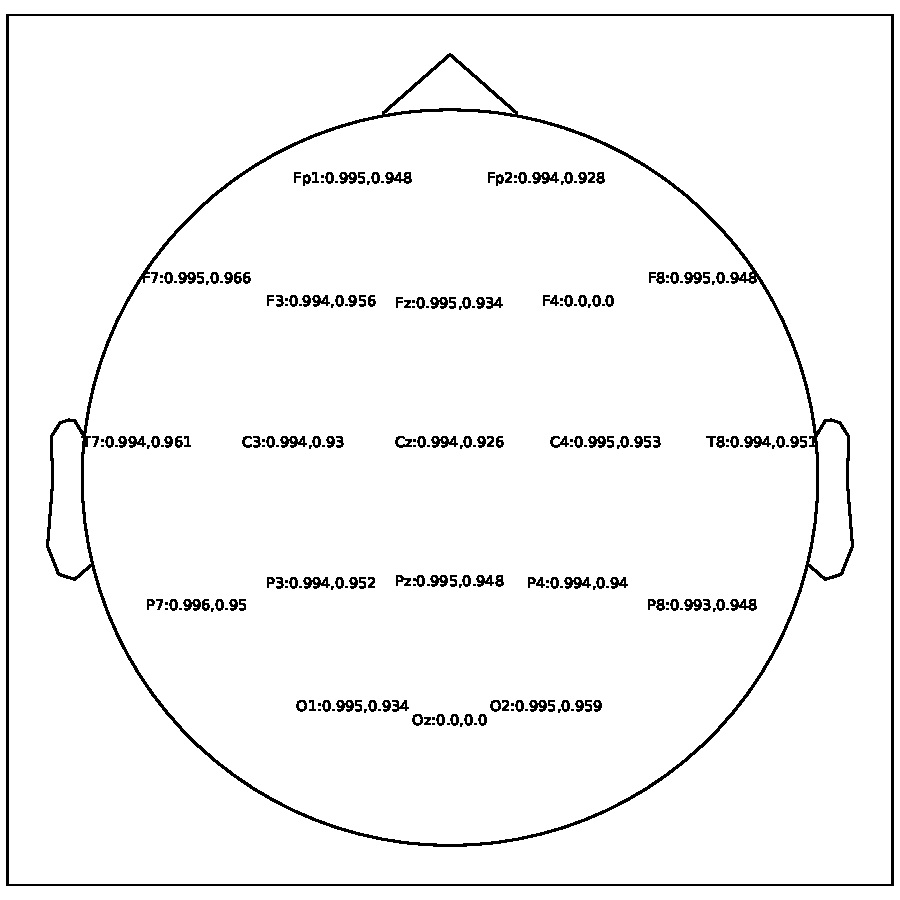
\includegraphics[width=.95\textwidth,trim={0cm 0cm 0cm 0cm},clip]{../SearchResults_3Ch/SearchSpaceResult_3Ch_(61_35)_S50_RemoveBaseLineOff_20191011}};
	  \begin{scope}[scale=1]
	      \draw[line width=2pt,blue] (-7.85,-7.85) node[anchor=west,right=.15cm] {\small{Best Channels according to the train accuracy}} circle (.2);
	      \draw[line width=2pt,red]  (7.85,-7.85)  node[anchor=east,left=.15cm] {\small{Best Channels according to the test accuracy}}  circle (.2);
	      %
	      %\draw[line width=2pt,blue] (-.2,-5.1) node[] (OzTr) {} circle (.45);
 	      %\draw[line width=2pt,blue] (1.65,-4.85) node[] (O2Tr) {} circle (.45);
 	      %\draw[line width=2pt,blue] (-6.1,.15) node[] (T7Tr) {} circle (.45);
	      %\draw[line width=2pt,blue] (-.25,.15) node[] (CzTr) {} circle (.45);
	      \draw[line width=2pt,blue] (2.75,.15) node[] (C4Tr) {} circle (.45);
	      %\draw[line width=2pt,blue] (-3.2,.15) node[] (C3Tr) {} circle (.45);
	      %\draw[line width=2pt,blue] (-2.05,-4.9) node[] (O1Tr) {} circle (.45);
 	      %\draw[line width=2pt,blue] (5.75, .15) node[] (T8Tr) {} circle (.45);
	      %\draw[line width=2pt,blue] (4.6, 3.25) node[] (F8Tr) {} circle (.45);
	      %\draw[line width=2pt,blue] (2.2, 2.85) node[] (F4Tr) {} circle (.45);
	      %\draw[line width=2pt,blue] (-.25, 2.8) node[] (FzTr) {} circle (.45);
	      \draw[line width=2pt,blue] (-5., -2.95) node[] (P7Tr) {} circle (.45);
	      %\draw[line width=2pt,blue] (-2., 5.2) node[] (PF1Tr) {} circle (.45);
	      %\draw[line width=2pt,blue] (1.7, 5.2) node[] (PF2Tr) {} circle (.45);
	      %\draw[line width=2pt,blue] (4.6, -2.95) node[] (P8Tr) {} circle (.45);
	      %\draw[line width=2pt,blue] (-2.7, -2.5) node[] (P3Tr) {} circle (.45);
	      \draw[line width=2pt,blue] (-.25, -2.5) node[] (PzTr) {} circle (.45);
	      %
	      %\draw[line width=2pt,red] (.6,2.8) node[] (FzTe) {} circle (.45);
	      %\draw[line width=2pt,red] (3.1, 2.85) node[] (F4Te) {} circle (.45);
	      %\draw[line width=2pt,red] (3.1,-2.5) node[] (P4Te) {} circle (.45);
	      %\draw[line width=2pt,red] (.6,-2.5) node[] (PzTe) {} circle (.45);
	      %\draw[line width=2pt,red] (5.45,-2.95) node[] (P8Te) {} circle (.45);
	      %\draw[line width=2pt,red] (2.55,5.2) node[] (FP2Te) {} circle (.45);
	      %\draw[line width=2pt,red] (5.45, 3.25) node[] (F8Te) {} circle (.45);
	      \draw[line width=2pt,red] (-4.15, 3.25) node[] (F7Te) {} circle (.45);
	      %\draw[line width=2pt,red] (-1.25, -4.85) node[] (O1Te) {} circle (.45);
	      \draw[line width=2pt,red] (2.65, -4.85) node[] (O2Te) {} circle (.45);
	      %\draw[line width=2pt,red] (-2.3, .15) node[] (C3Te) {} circle (.45);
	      %\draw[line width=2pt,red] (.65, .15) node[] (CzTe) {} circle (.45);
 	      %\draw[line width=2pt,red] (2.8+1, .15) node[] (C4Te) {} circle (.45);
	      %\draw[line width=2pt,red] (6.6, .15) node[] (T8Te) {} circle (.45);
		\draw[line width=2pt,red] (-5.1, .15) node[] (T7Te) {} circle (.45);
 	      %\draw[line width=2pt,red] (.7, -5.1) node[] (OzTe) {} circle (.45);
	\end{scope}
  \end{tikzpicture}
  \caption{Search for the third best channel with $50$ subjects, no baseline is removed.}
  \label{fg:3Ch_S50_B0}
\end{figure}




\end{document}